\documentclass[ xcolor = pdftex, dvipsnames, table ]{beamer}

\usetheme[compress]{Berlin}
\usecolortheme{whale}
\setlength{\parskip}{0.1in}
%
\usepackage{bm}
\usepackage{graphicx}
\usepackage{amsmath}
\usepackage{amssymb}
\usepackage{relsize}
\usepackage{dsfont}
%
\usepackage{multimedia}
\usepackage{media9}
\usepackage{attachfile2}
%
\newcommand{\includemovie}[2][]{
    \includemedia[
        #1,
        activate=pageopen,transparent,
        addresource=#2.mp4,addresource=#2.png,
        flashvars={
            file=#2.mp4&image=#2.png&
            stretching=uniform&start=0&
            screencolor=white& %improves render in light backgrounds
            controlbar.position=over&controlbar.idlehide=true&
            autostart=true&repeat=always&smoothing=true
            %&bufferlength=10 % may improve repetition of short videos
        }
    ]{ % for disabled content (in most cases this is fallback)
        \begin{tabular}{ll}
            \mbox{
            %   \href{run:#2.mp4} % for not embedded fallback
                \textattachfile[color={0 0 0}]{#2.mp4} % for embedded fallback
                {\texttt{|\kern-.23em>}} % poor play button
            } & \raisebox{-\height}{\includegraphics[#1]{#2}}
        \end{tabular}
    }{player.swf}
}
%
\newcommand{\E}[1]{
        \mathbb{E}\left[~#1~\right]
}
%
\DeclareMathOperator*{\argmin}{\arg\!\min}
\DeclareMathOperator*{\argmax}{\arg\!\max}
%

\def \Eix {
        \mathbb{E}\left[~\text{I}(\bm{x})~\right]
}

\def \EIx {
        \mathbb{E}\left[~\text{I}(\underline{\bm{x}})~\right]
}

\def \Ix {
        \text{I}(\underline{\bm{x}})
}

\def \ix {
        \text{I}(\bm{x})
}

\def \oner {
        \mathlarger{\mathds{1}}
}

\title{Assessing Convergence in Gaussian Process Surrogate Model
Optimization}
\author[]{Nick Grunloh\\ 
as advised by Dr. Herbie Lee
}% \vspace*{-0.2in}}
\institute[]{\textit{Applied Mathematics and Statistics \\  
University of California, Santa Cruz}
\vspace*{0.1in} \\
grunloh@soe.ucsc.edu\\
herbie@ucsc.edu
}

\begin{document}
\begin{frame}
\titlepage
\end{frame}

%
%

\section{Numerical Optimization}
\subsection{}
\begin{frame}{Optimization can be Tricky}
%\hspace{-1cm}
\begin{minipage}[h!]{0.6\textwidth}
%
\begin{equation*}
\argmin_{\bm{x}} f(\bm{x}) 
\end{equation*}
%
Problems:
\begin{itemize}
\item $\bm{x}$ may be in many dimensions
\item $f$ may be poorly behaved
\item Often no useful $f'$ information
\item $f$ evaluations may be expensive
\end{itemize}
%
$~$\\
Example:\\
Computer simulation experiments
%
\end{minipage}
\begin{minipage}[h!]{0.38\textwidth}
%
\movie[autostart, loop, poster, height=0.45\textheight,width=\textwidth]{}{compSim.mp4}
%
\end{minipage}
\end{frame}

%
%

\subsection{}
\begin{frame}{Newton-Raphson}
%
\begin{center}
\vspace{-0.4cm}
\movie[autostart, loop, poster, height=0.84\textheight, width=0.85\textwidth]{}{newtonRaphson.mp4}
\end{center}
%
\end{frame}

%
%

\begin{frame}{Beyond Newton-Raphson: Pattern Search}
%
\begin{center}
\movie[autostart, loop, poster, height=0.8\textheight, width=0.6\textwidth]{}{patternSearch.mp4}
\end{center}
%
\end{frame}

%
%

\begin{frame}{Beyond Newton-Raphson: Simulated Annealing}
%
\begin{center}
\movie[autostart, loop, poster, height=0.45\textheight, width=\textwidth]{}{simAnnealing.mp4}
\end{center}
%
\end{frame}

%
%

\begin{frame}{Beyond Newton-Raphson: Evolutionary Algorithms}
%
\begin{center}
\vspace{-0.3cm}
\movie[autostart, loop, poster, height=0.85\textheight, width=0.625\textwidth]{}{gaSearching.mp4}
\end{center}
%
\end{frame}

%
%

\subsection{}
\begin{frame}{Statistical Surrogate Modeling}
%
\begin{minipage}[h!]{0.49\textwidth}
Procedure:
\begin{itemize}
        \item[1)] Collect an initial set\\
		 from the domain $\bm{x}$
        \item[2)] Compute $f(\bm{x})$
        \item[3)] Model $f$
        \item[4)] Predict an optimal $\bm{x^*}$
	\item[4)] Add $\bm{x^*}$ to $\bm{x}$
        \item[5)] Check convergence
        \item[6)] If converged exit.\\
		 Otherwise go to 2).
\end{itemize}
\end{minipage}
\begin{minipage}[h!]{0.49\textwidth}
	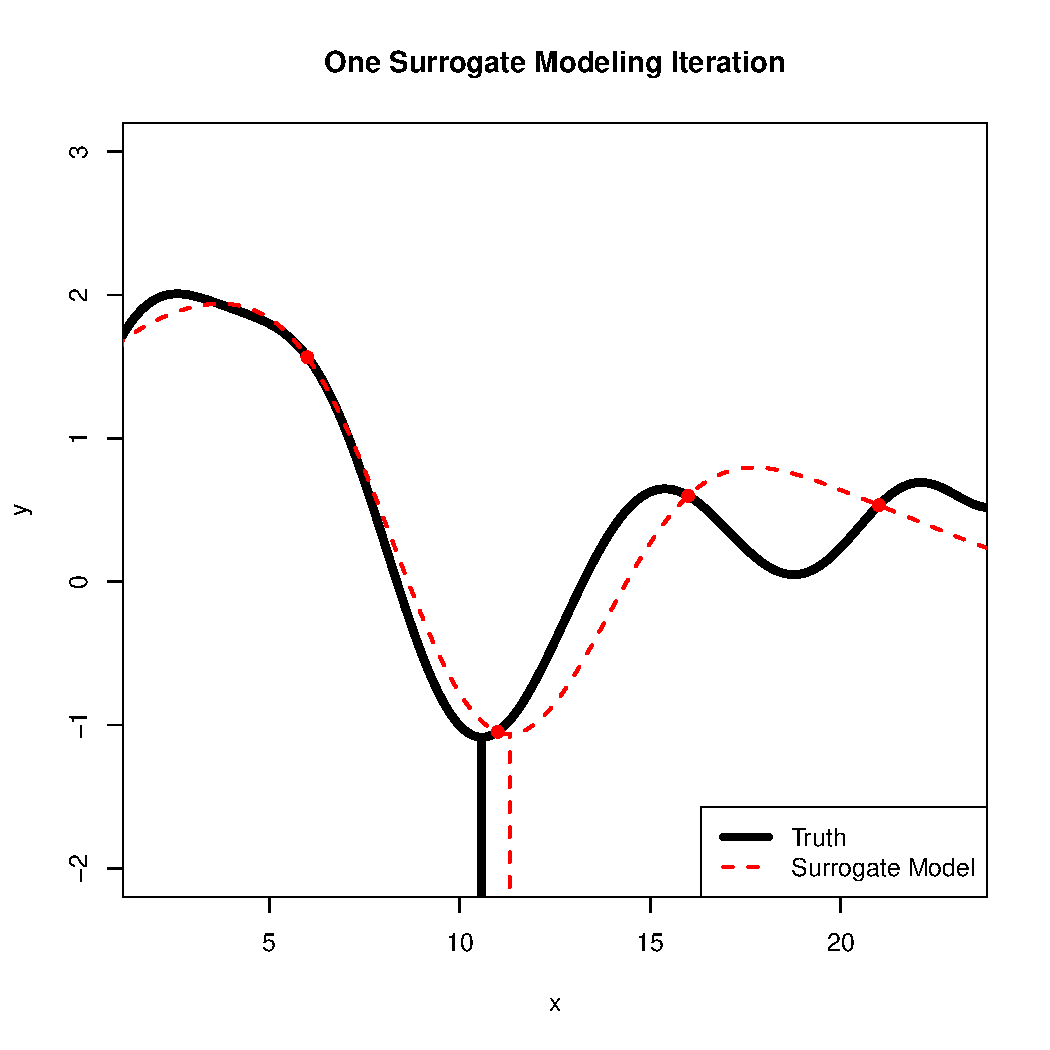
\includegraphics[width=\textwidth]{surrogateStep.pdf}
\end{minipage}
\end{frame}

%
%

\begin{frame}{Treed GP Surrogate Model}
\begin{minipage}[h!]{0.55\textwidth}
\vspace{0.5cm}
Partition $f$ across $R$ regions:
\begin{align*}
f_{r} &\sim \text{GP}\left( m_{r}(\bm{x}), C_{r}(\bm{x}, \bm{x'})\right)\\
\cup_{r=1}^{R} f_r &= f\\
&\\
f &\sim \mathcal{T}\text{GP}
\end{align*}
Hierarchical priors for $m_{r}(.)$ and $C_{r}(.)$ parameters to share across partitions.
\end{minipage} 
\begin{minipage}[h!]{0.43\textwidth}
%\vspace{0.1cm}
\begin{center}
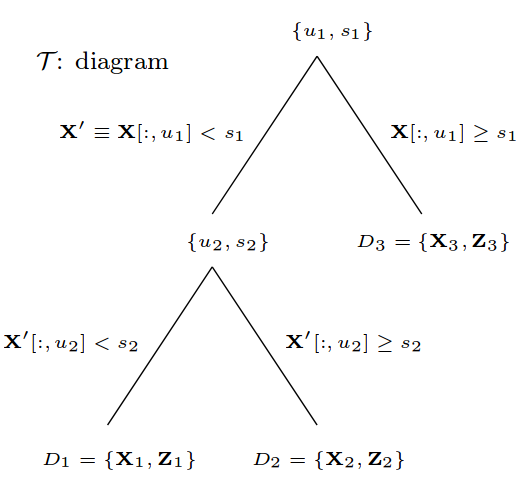
\includegraphics[height=0.5\textwidth]{tree.png}\\
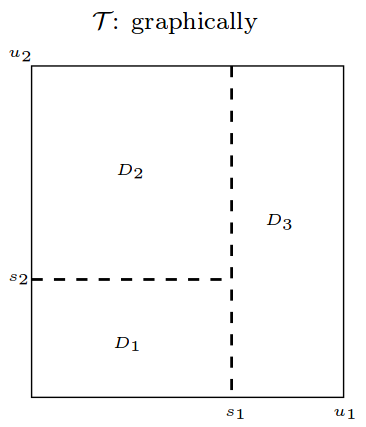
\includegraphics[height=0.7\textwidth]{parts.png}
\end{center}
\end{minipage}

%\vspace{-0.3cm}
\scalebox{0.6}{*} \scalebox{0.6}{ R. B. Gramacy, (2007). {\em tgp: An R Package for Bayesian Nonstationary, Semiparametric Nonlinear}}\\
\vspace{-0.2cm}
\scalebox{0.6}{ {\em Regression and Design by Treed Gaussian Process Models}. Journal of Statistical Software, 19(9), 1-46.} 
%\item R. B. Gramacy, \& H. K. Lee. (2008). {\em Bayesian treed Gaussian process models with an application to computer modeling}. Journal of the American Statistical Association, 103, 1119-1130.
%\item R. B. Gramacy, \& M. Taddy (2010). {\em Categorical Inputs, Sensitivity Analysis, Optimization and Importance Tempering with tgp Version 2, an R Package for Treed Gaussian Process Models}. Journal of Statistical Software, 33(6), 1-48.
%\begin{itemize}
%	\item Flexible
%	\item good predictive framework for optimal(in some sense) search
%\end{itemize}
\end{frame}

%
%

%\begin{frame}{\color{red}partitioned GP}
%\begin{itemize}
%	\item Even more Flexible
%	\item pictures to demonstrate
%	\item R package TGP
%\end{itemize}
%\end{frame}

%
%

\begin{frame}{Expected Improvement (EI)}
\begin{minipage}[h!]{0.49\textwidth}
\begin{align*}
	f_{min} &= \min\Big\{ f(\bm{x_1}), ..., f(\bm{x_{N}}) \Big\}\\
        \ix &= \max \Big\{ \big(f_{min} - f(\bm{x})\big), ~0 \Big\}\\
        \text{EI} &= \Eix
\end{align*}
\end{minipage}
\begin{minipage}[h!]{0.49\textwidth}
\begin{center}
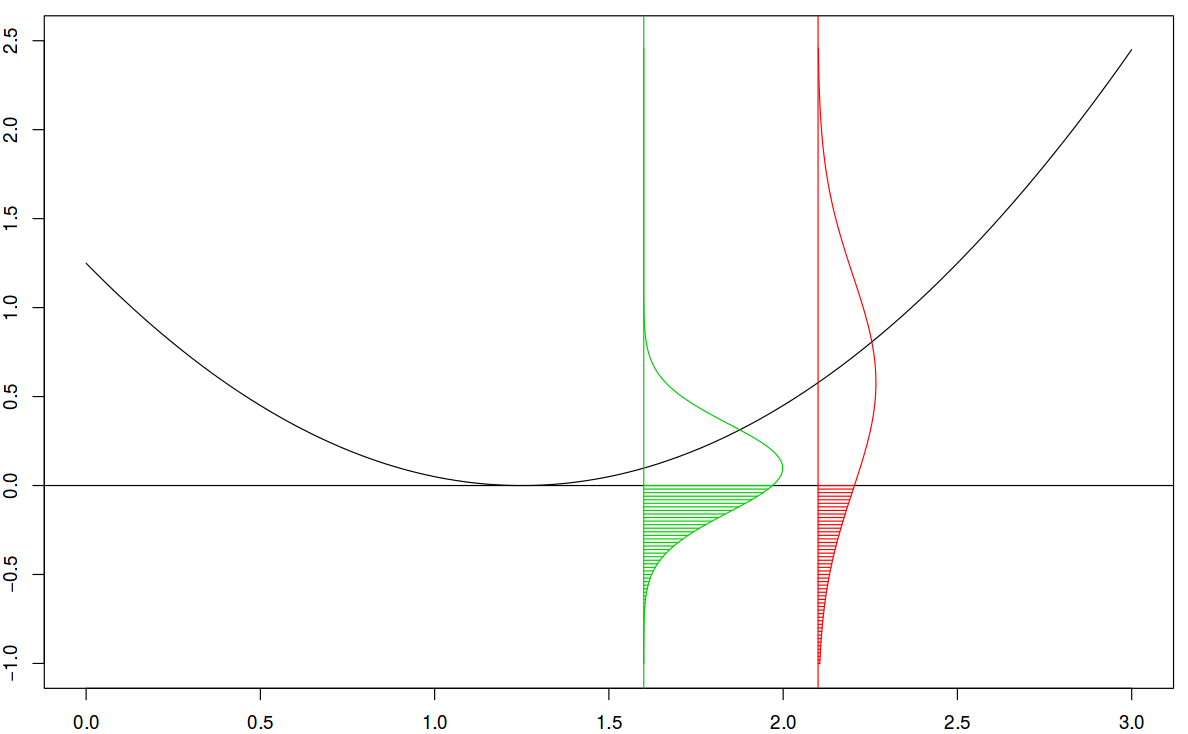
\includegraphics[width=\textwidth]{eiPic.png}
\end{center}
\end{minipage}
%\begin{itemize}
%	\item EI criterion formula
%	\item EI Intuition
%	\item EI Uncertainty Herbie Picture
%\end{itemize}
\end{frame}

%
%

\section{Convergence}
\subsection{}
\begin{frame}{Convergence}
%\hspace{-1cm}
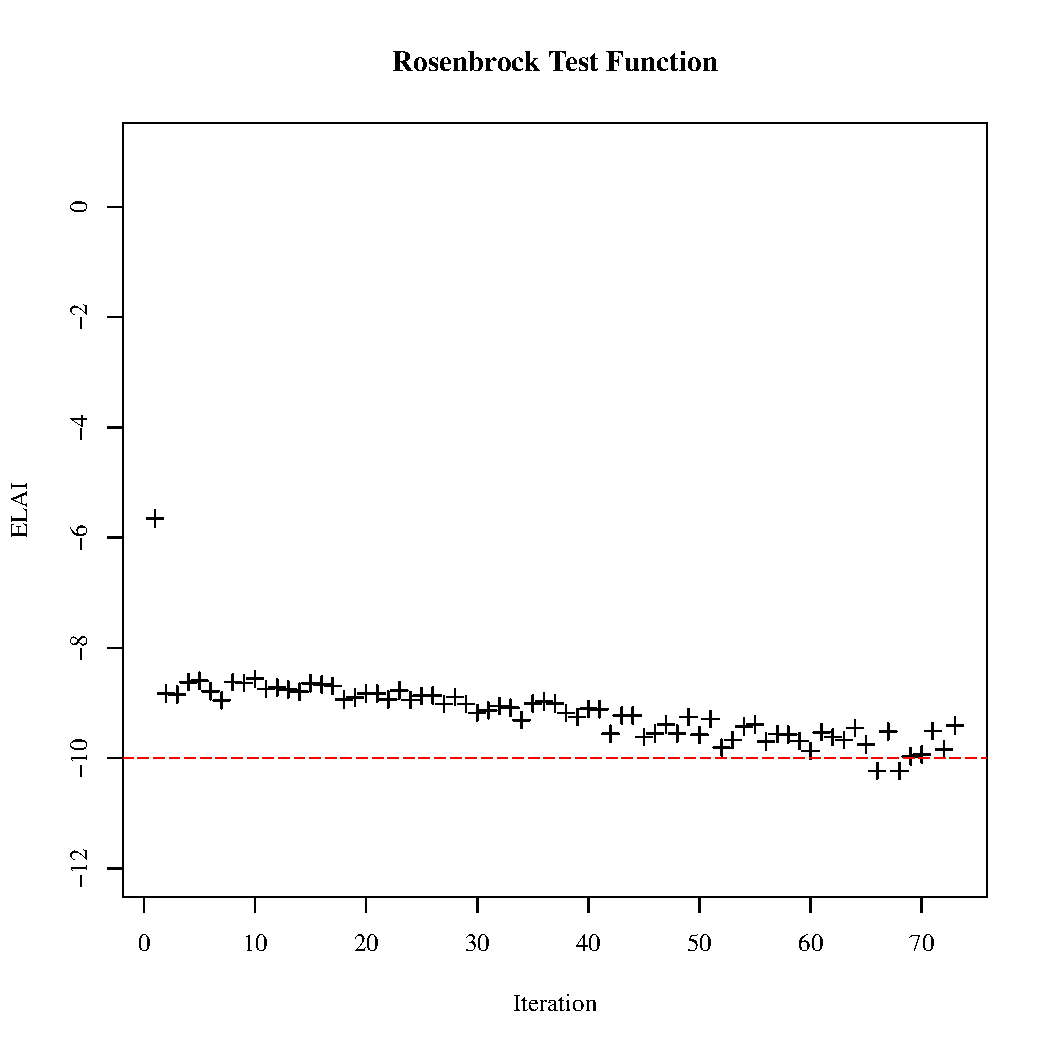
\includegraphics[width=0.33\textwidth]{introChartRoseEasyEasyAxis.pdf}
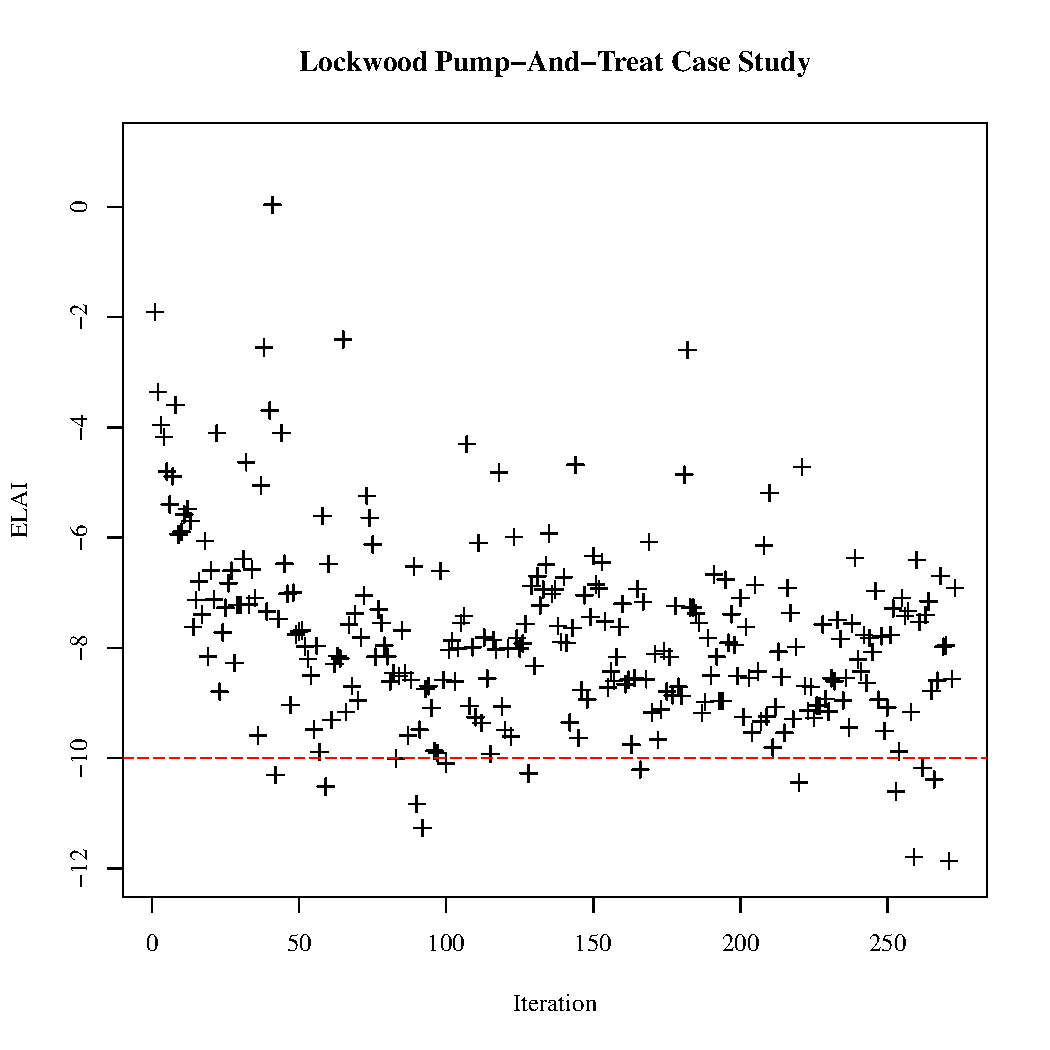
\includegraphics[width=0.33\textwidth]{introChartLock6Three20000Axis.pdf}
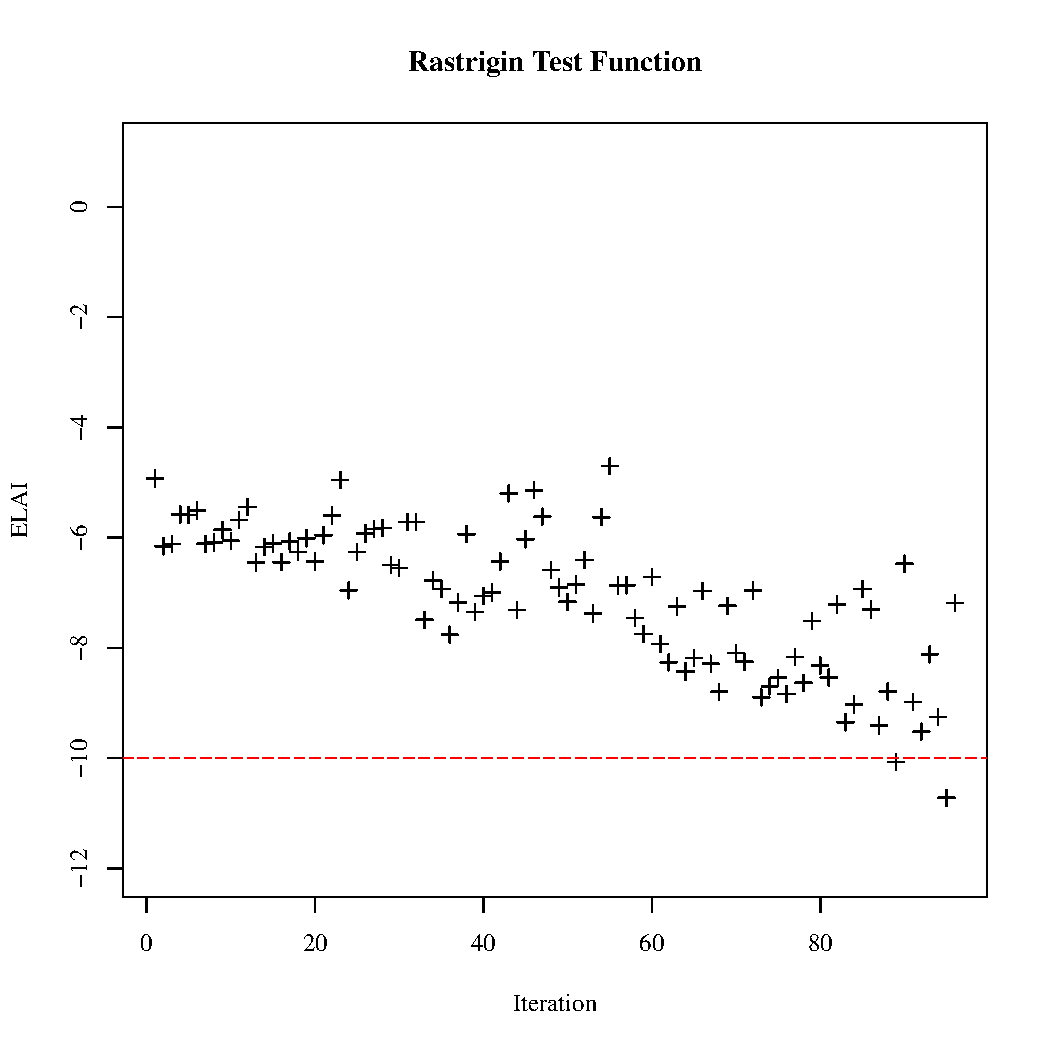
\includegraphics[width=0.33\textwidth]{introChartRastHardAxis.pdf}
%\begin{itemize}
%	\item Convergence Drifts
%	\item Hypothetical Drift pattern
%	\item Improvement Distribution is far from normal (picture)
%	\item KISS (when possible)
%	\item Not much love from these data
%\end{itemize}
\end{frame}

%
%

\subsection{}
\begin{frame}{Statistical Process Control (SPC)}
%
\hspace{-0.7cm}
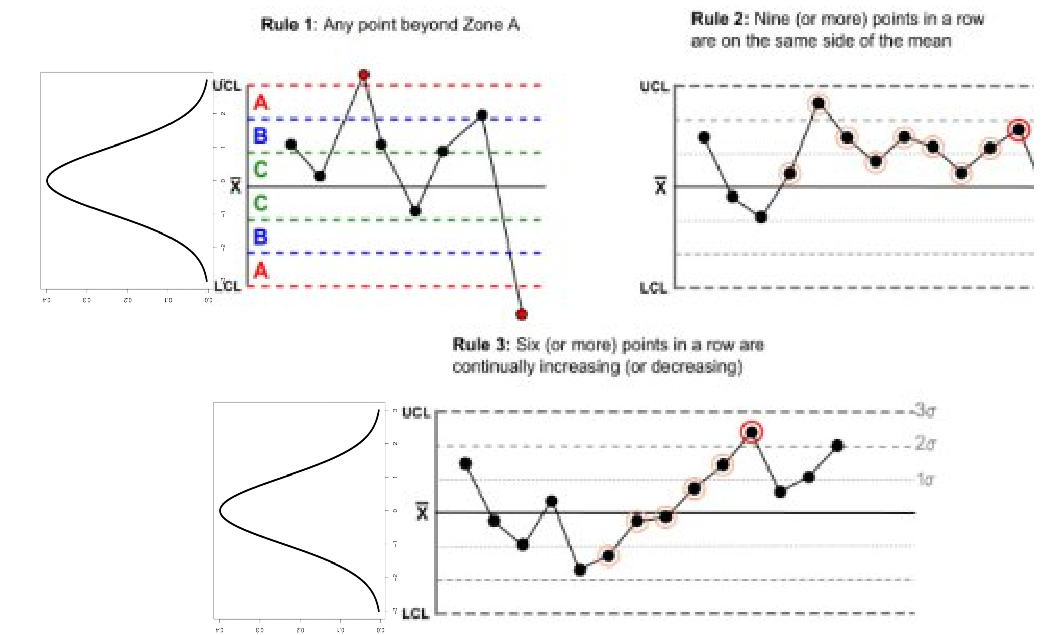
\includegraphics[width=\textwidth]{spcComp.pdf}
%
%\begin{itemize}
%	\item X-bar Chart Shewhart 1920
%	\item repeated sampling story
%	\item confidence intervals as control limits
%\end{itemize}
\end{frame}

%
%

\subsection{}
\begin{frame}{Convergence is Subtle}
\vspace{0.5cm}
\begin{minipage}[h!]{0.6\textwidth}
\begin{align*}
	\hspace*{-1cm}
	z_i &= \lambda \bar x_i+(1-\lambda)z_{i-1}\\
	\sigma^2_{z_i} &= \frac{{\sigma^2_x}}{n} \left(\frac{\lambda}{2-\lambda}\right)\left[1-(1-\lambda)^{2i}\right]\\
	&\\
	\text{CL}_i &=  \mu \pm c ~ \sigma_{z_i}
\end{align*}
\end{minipage}
\begin{minipage}[h!]{0.38\textwidth}
\begin{center}
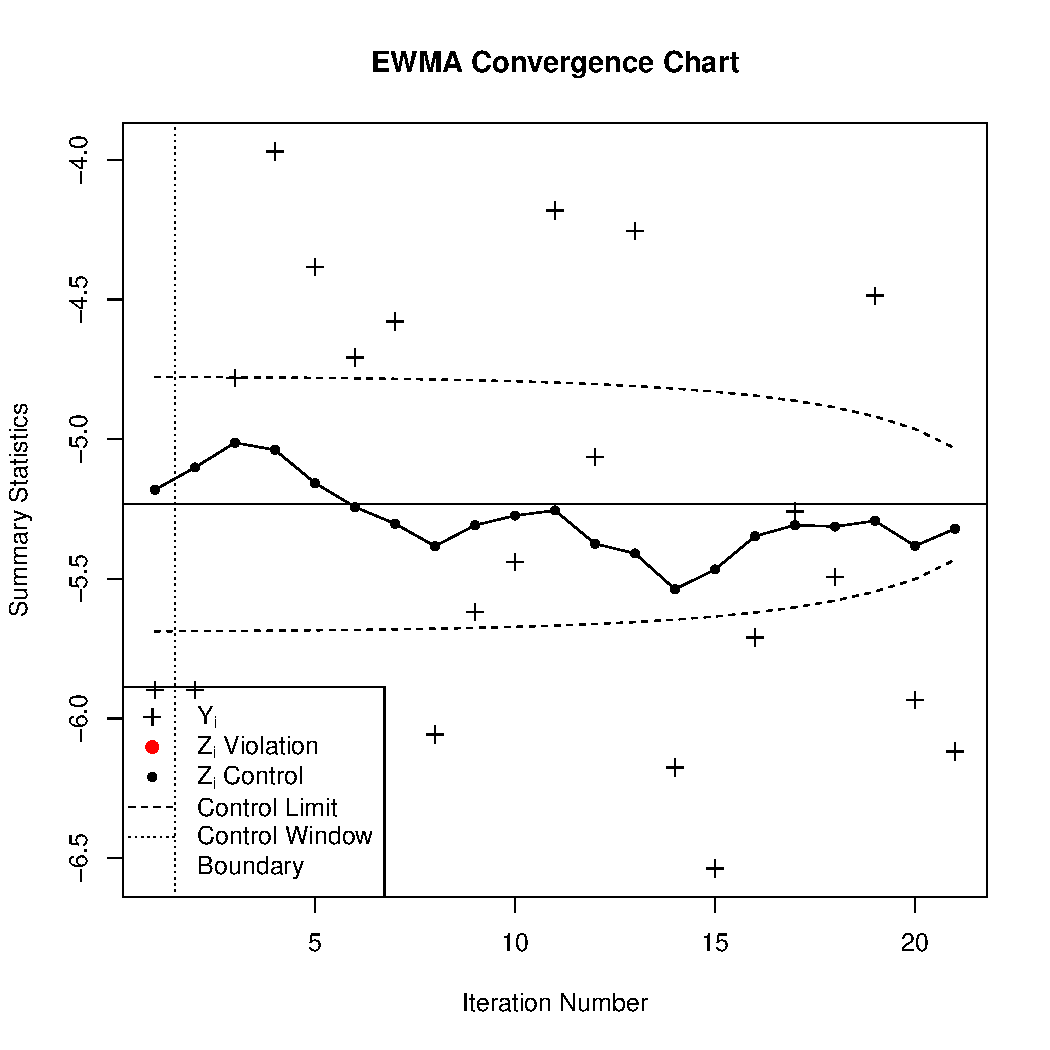
\includegraphics[width=\textwidth]{ewmaConvChartEasomMedStart.pdf}
\end{center}
\end{minipage}

\vspace{0.5cm}
\scalebox{0.7}{*} \scalebox{0.7}{L. Scrucca (2004). {\em qcc: an R package for quality control charting and statistical process}} \scalebox{0.7}{ {\em control}. R News 4/1, 11-17.}
%%
%\begin{minipage}[h!]{0.7\textwidth}
%\begin{align*}
%z_i &= \lambda \bar x_i+(1-\lambda)z_{i-1}\\
%\sigma^2_{z_i} &= \sigma^2_{\bar x_i} \left(\frac{\lambda}{2-\lambda}\right)\left[1-(1-\lambda^{2i})\right]\\
%\text{CL}_i &=  \mu \pm c ~ \frac{\sigma_x}{\sqrt{n}}~\sqrt{\left(\frac{\lambda}{2-\lambda}\right)\left[1-(1-\lambda^{2i})\right]}
%\end{align*}
%\end{minipage}
%\begin{minipage}[h!]{0.29\textwidth}
%%
%Foo
%%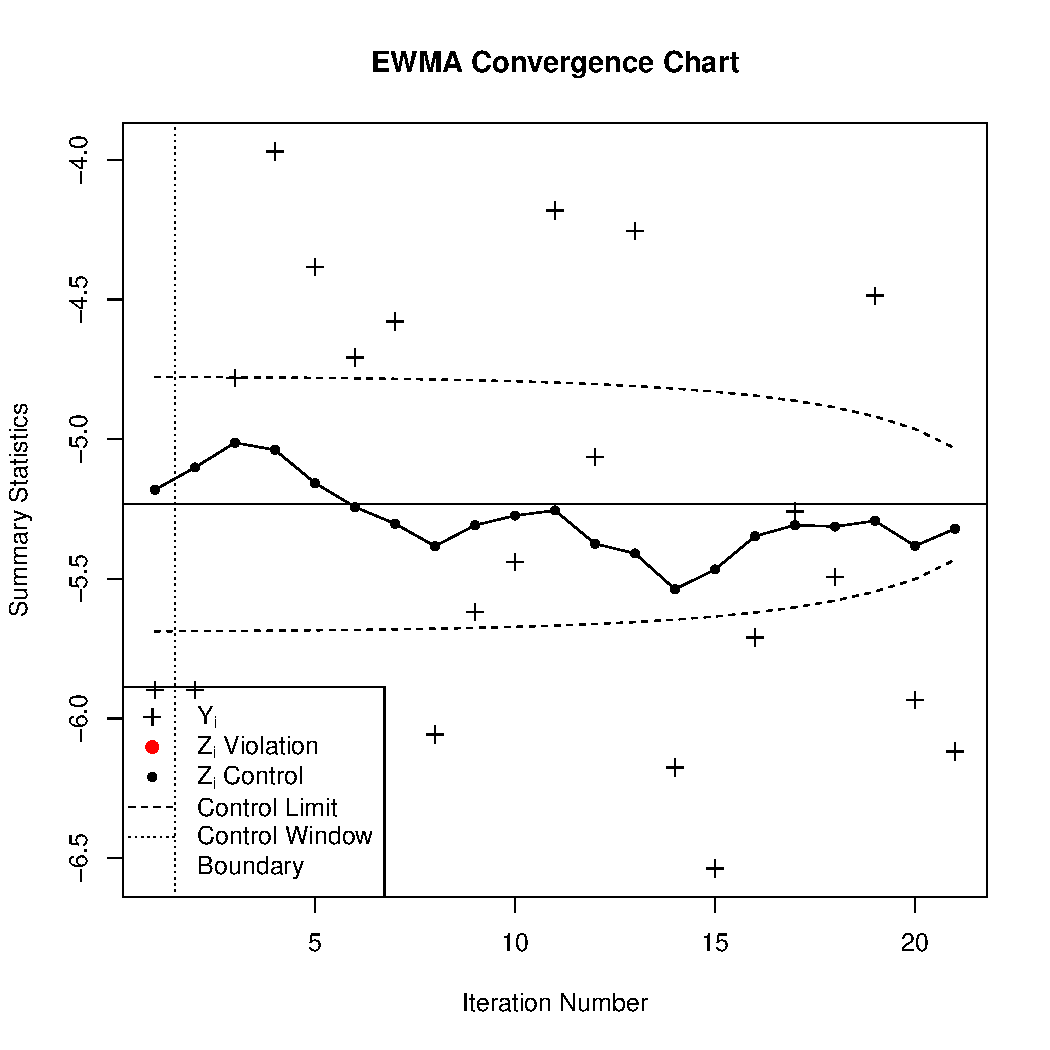
\includegraphics[width=0.5\textwidth]{ewmaConvChartEasomMedStart.pdf}
%%
%\end{minipage}
%%
%
%%\begin{itemize}
%%	\item SPC via EWMA 
%%	\item smoothing criterion
%%	\item control limit differences (formula)
%%	\item Normality assumption grrr :/
%%\end{itemize}
\end{frame}

%
%

%\subsection{}
%\begin{frame}{}
%%
%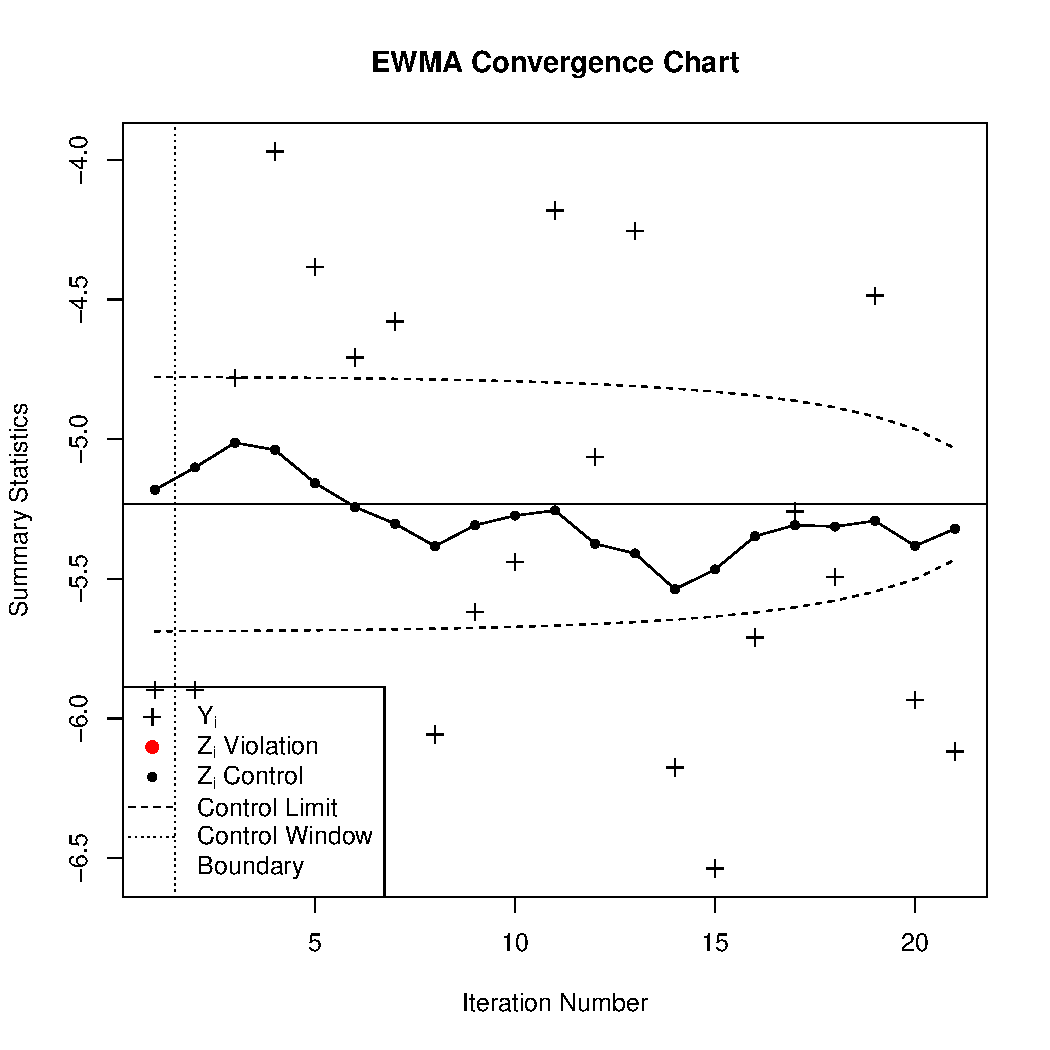
\includegraphics[width=\textwidth]{ewmaConvChartEasomMedStart.pdf}
%%
%\end{frame}


%\subsection{}
%\begin{frame}{Make it more normal (It gets a little messy)}
%\begin{itemize}
%	\item transform data (KISS log)
%	\item pre/post picture
%	\item MCMC samples contain 0's :)
%	\item why is this an issue
%\end{itemize}
%\end{frame}
%
%\subsection{}
%\begin{frame}{Model based log transformation}
%\begin{itemize}
%	\item ELAI in words
%	\item formula
%	\item Now we have a reliable criterion!
%\end{itemize}
%\end{frame}

\subsection{}
\begin{frame}{Build a Convergence Chart}
%\begin{minipage}[h!]{0.29\textwidth}
%\begin{itemize}
%	\item Choose $\lambda$
%	\item EWMA chart
%	\item Choose $w$
%\end{itemize}
%\end{minipage}
%\begin{minipage}[h!]{0.69\textwidth}
\begin{center}
\vspace{-0.5cm}
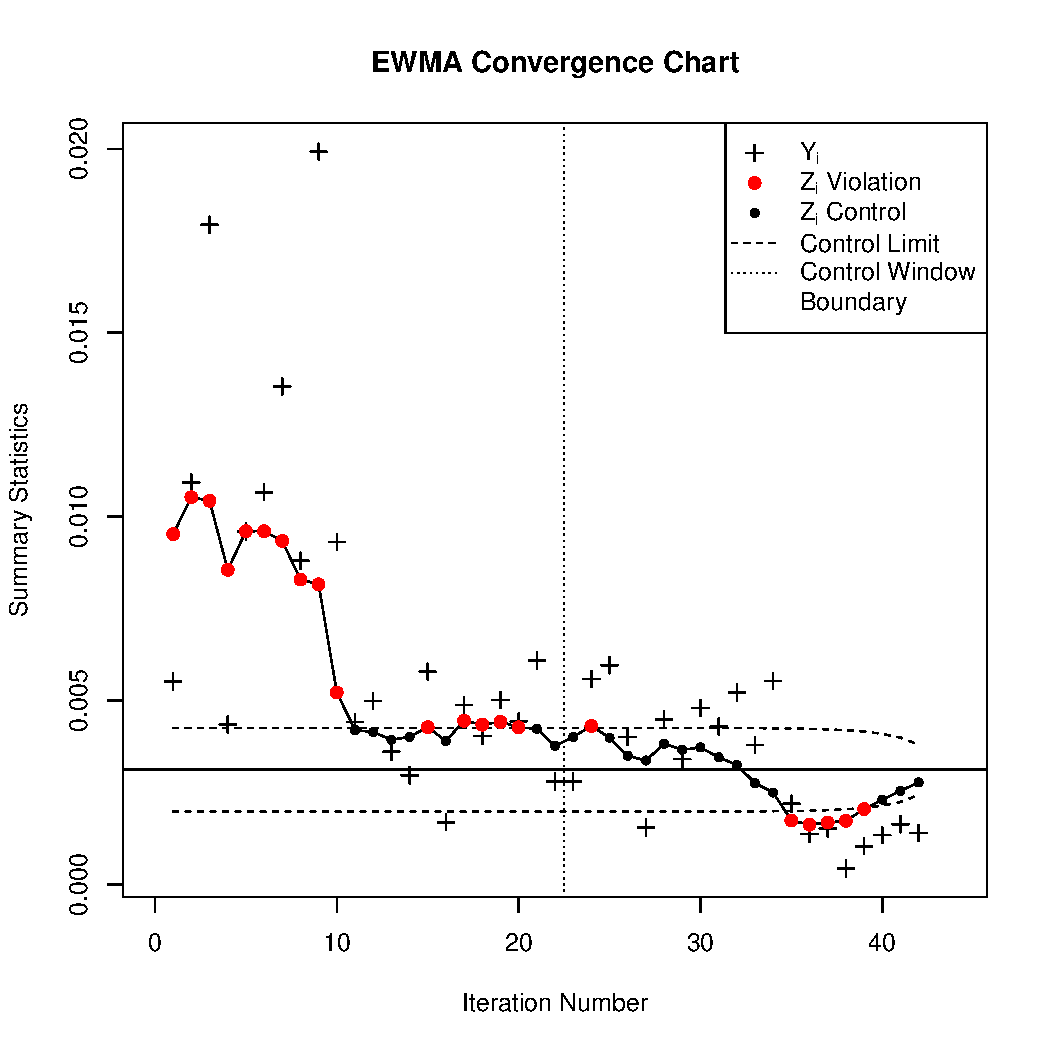
\includegraphics[height=0.9\textheight]{exampleEWMAM.pdf}
\end{center}
%\end{minipage}
%\begin{itemize}
%	\item build picture so far
%	\item control window
%	\item why we need this
%	\item how it works
%\end{itemize}
\end{frame}

%
%

\subsection{}
\begin{frame}{Interpret a Convergence Chart}	
\begin{center}
\vspace{-0.5cm}
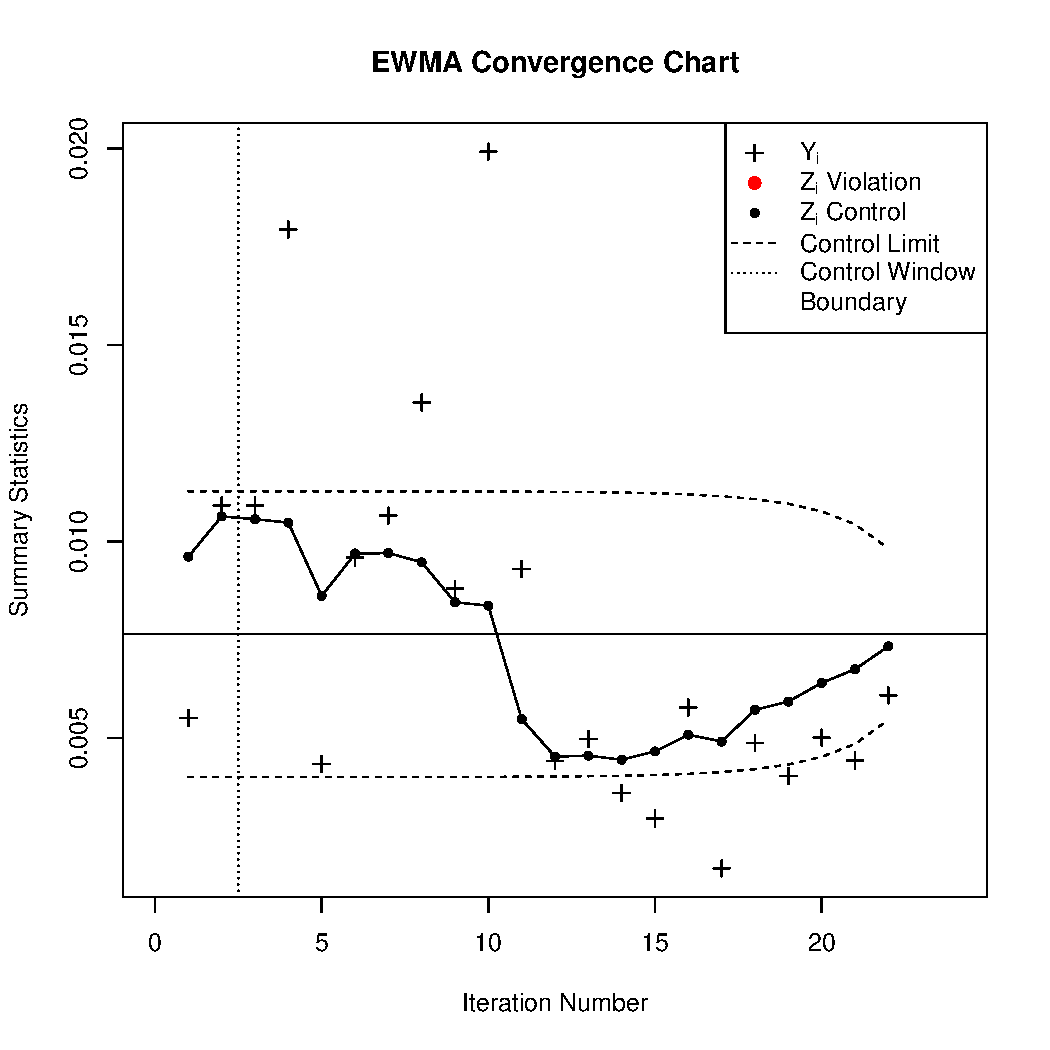
\includegraphics[width=0.33\textwidth]{exampleEWMAL.pdf}
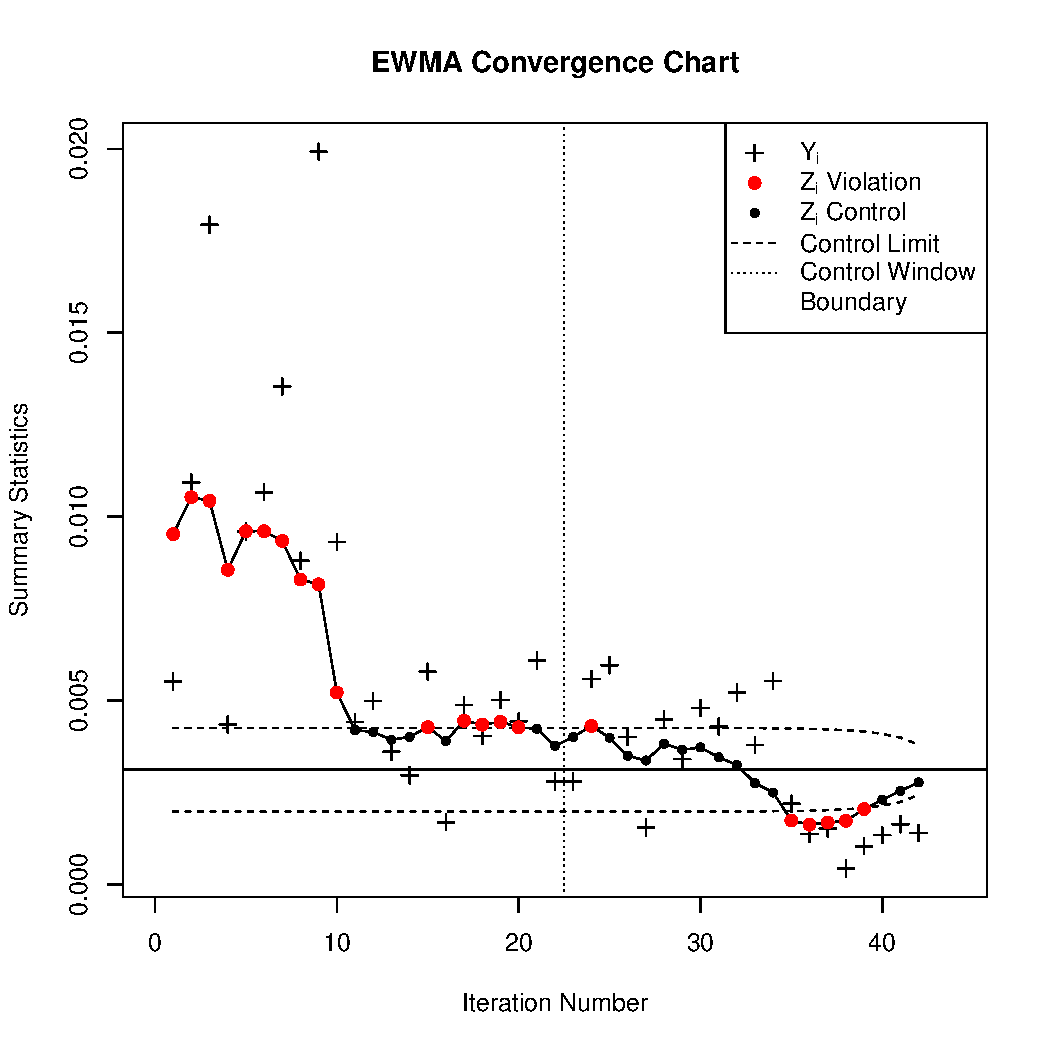
\includegraphics[width=0.33\textwidth]{exampleEWMAM.pdf}
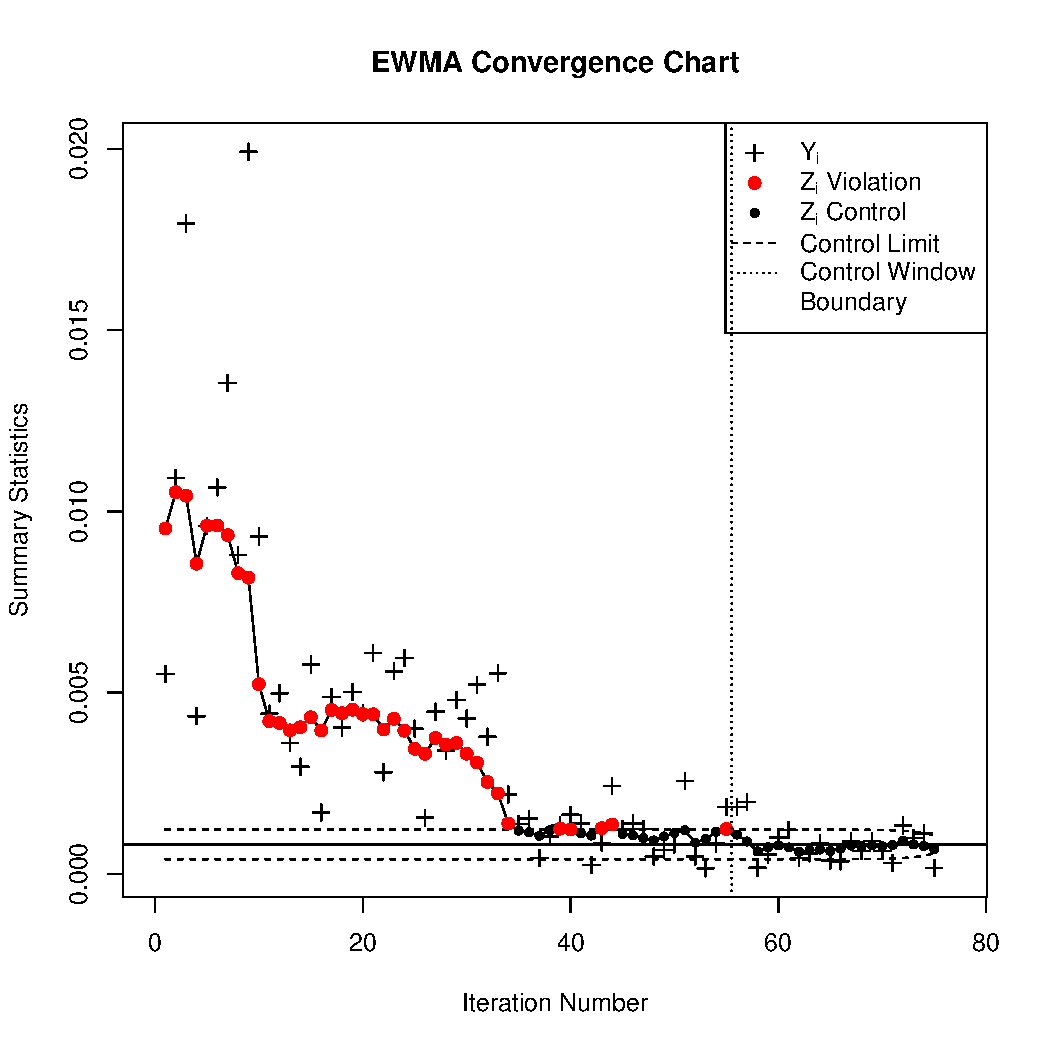
\includegraphics[width=0.33\textwidth]{exampleEWMAR.pdf}
\end{center}
%\begin{itemize}
%	\item control in the control window
%	\item out of control beyond window
%	\item Explain rules for identifying convergence
%	\item point out parameters $\lambda$ and $w$
%\end{itemize}
\end{frame}

%
%

\section{Examples}
\subsection{}
\begin{frame}{Rosenbrock Test Function}
\vspace{-0.3cm}
\begin{figure}[!h]%{l}{1.\textwidth}
        \centering
        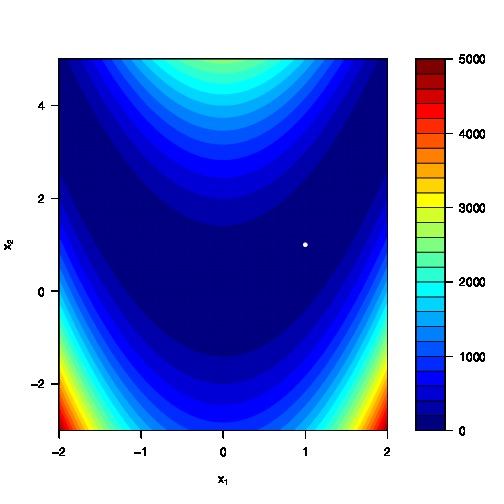
\includegraphics[width=0.49\textwidth]{roseContour.jpg}
        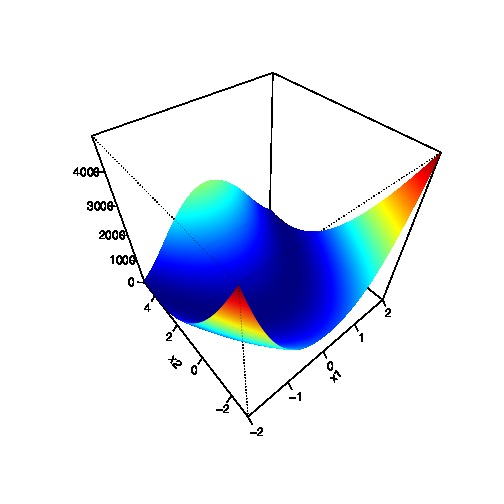
\includegraphics[width=0.49\textwidth]{rosePersp.jpg}
	\vspace{-0.5cm}
        \begin{eqnarray}
        f(x_1, x_2) &=& 100\left(x_2-x_1^2\right)^2 + (1-x_1)^2 \nonumber\\
        \text{Minimum}&:& f(1, 1)=0\nonumber
        \end{eqnarray}
\end{figure}
%\begin{itemize}
%	\item function and pictures
%	\item why its hard (classical test function)
%\end{itemize}
\end{frame}

%
%

\begin{frame}{Rosenbrock Pre-Convergence}
\begin{figure}[h!]%{l}{0.5\textwidth}
        %\hspace{-1cm}
        %\vspace{-0.2cm}
        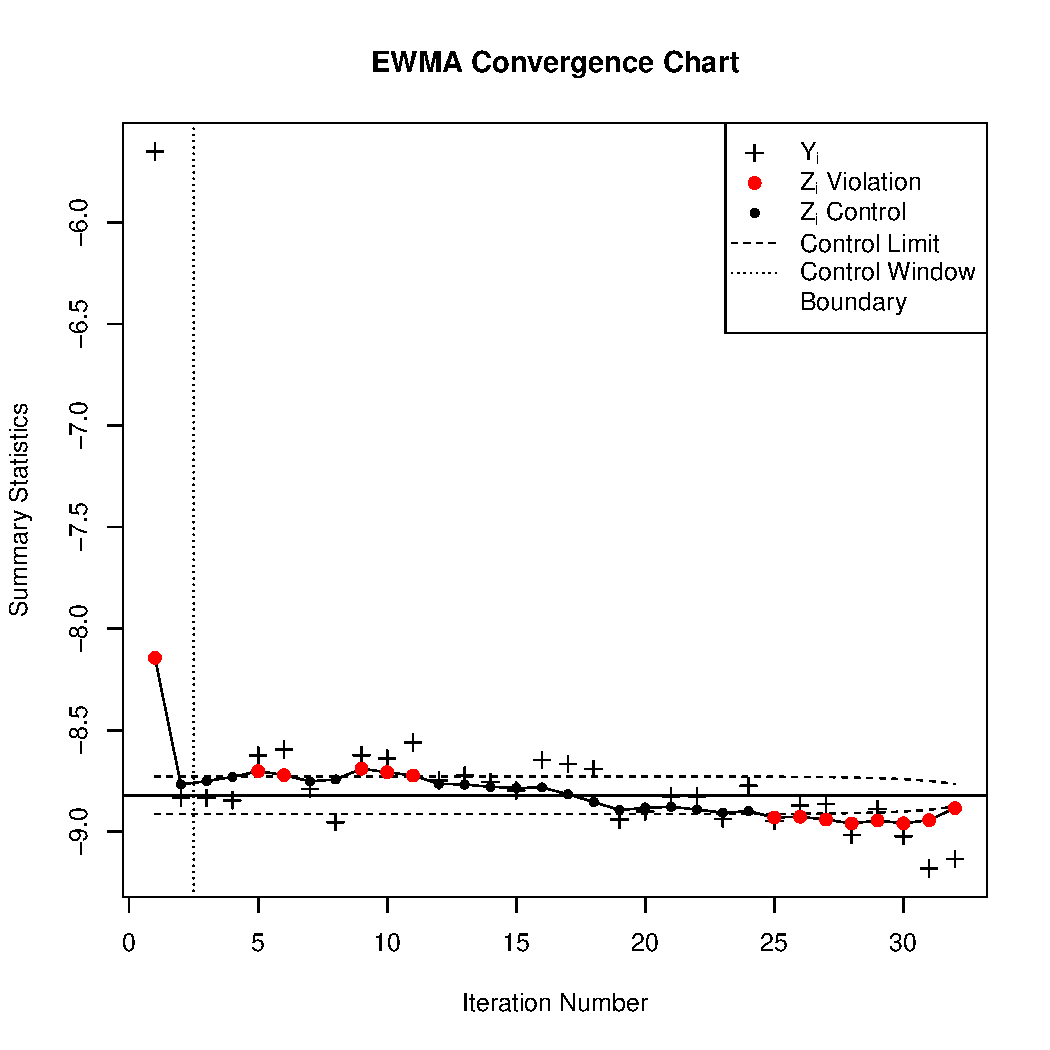
\includegraphics[width=0.49\textwidth]{ewmaConvChartRoseEasyEasyStart.pdf}
        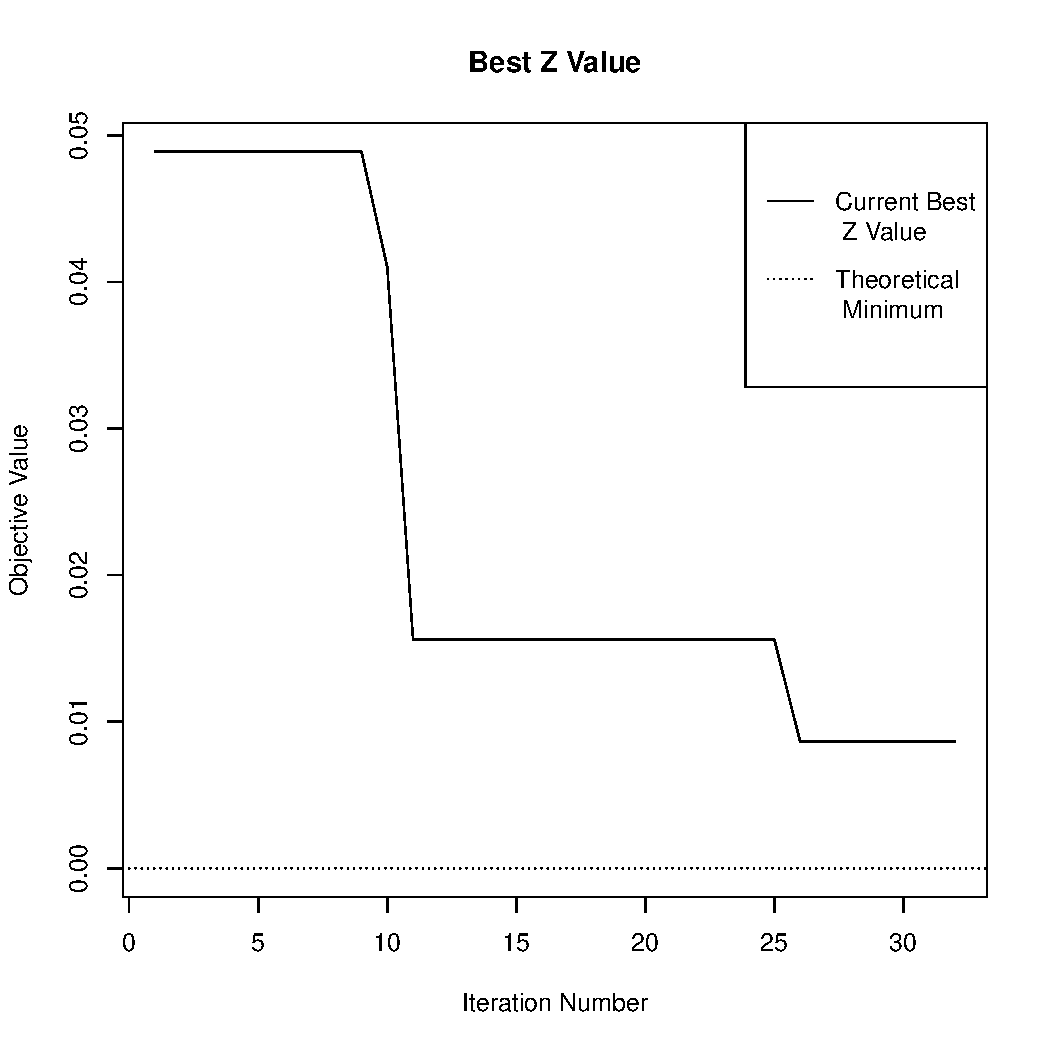
\includegraphics[width=0.49\textwidth]{bestZRoseEasyEasyStart.pdf}
	%\includegraphics[width=0.49\textwidth]{ewmaConvChartRoseEasyEasyEnd.pdf}
        %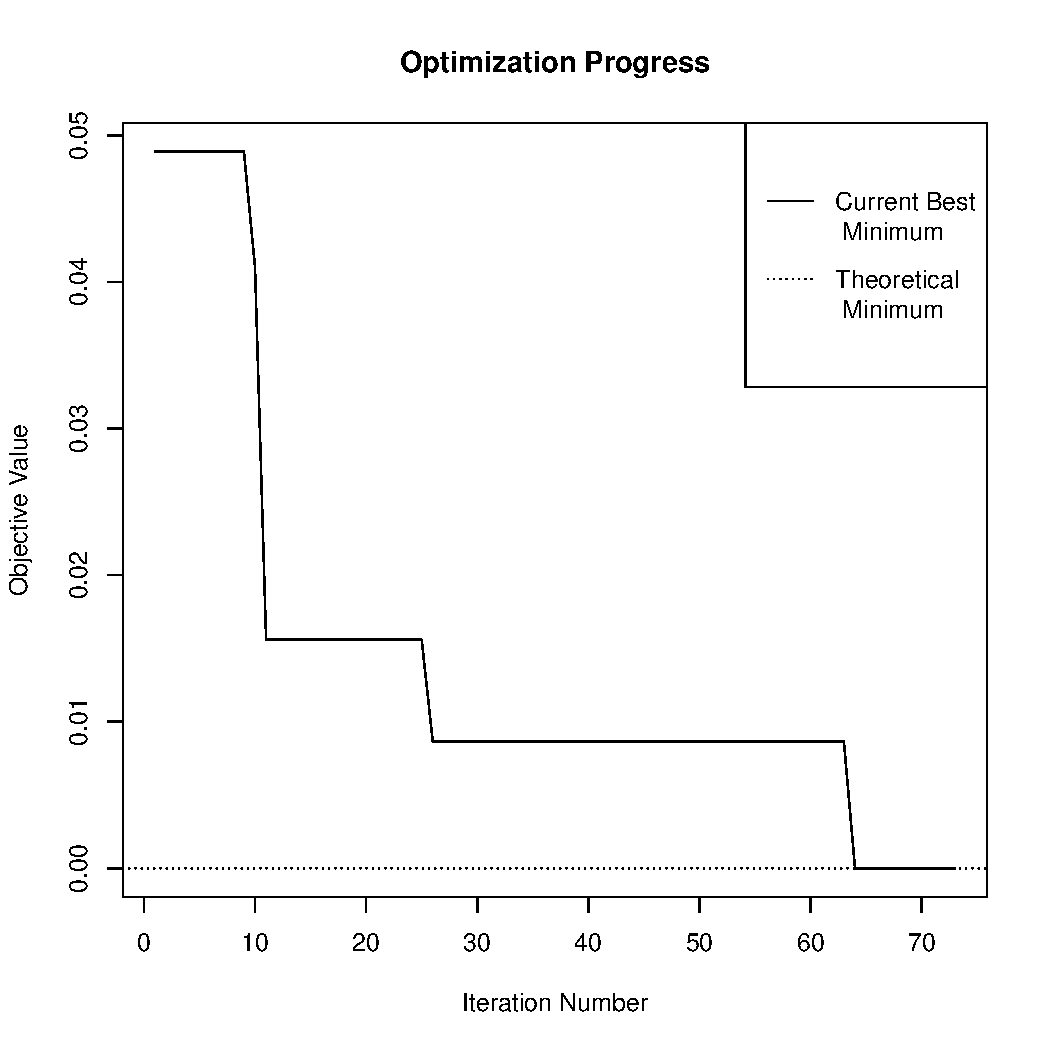
\includegraphics[width=0.49\textwidth]{bestZRoseEasyEasyEnd.pdf}
%       %\hspace{-1cm}
%       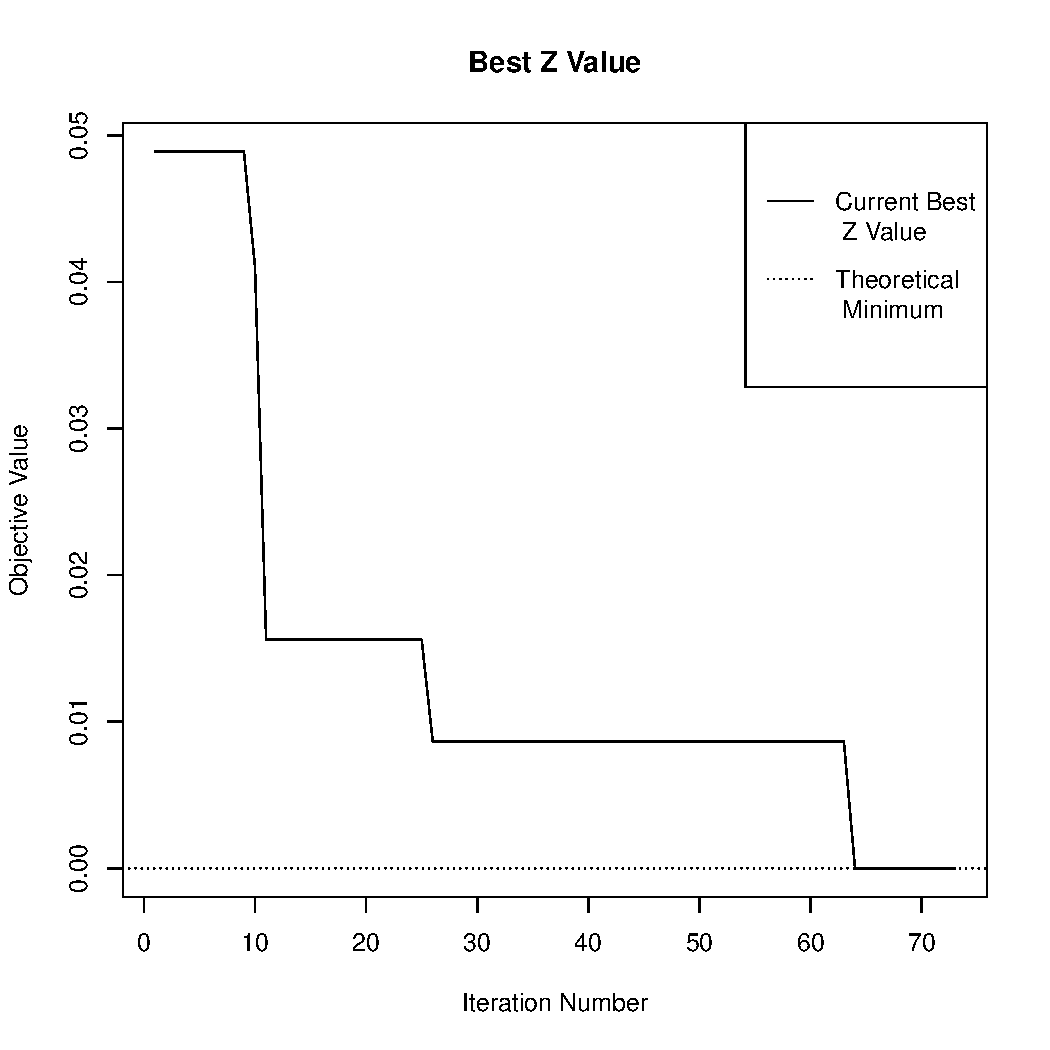
\includegraphics[width=0.245\textwidth]{./figures/bestZRoseEasyEasyEnd.pdf}
%       \includegraphics[width=0.245\textwidth]{./figures/ewmaConvChartRoseEasyEasyEnd.pdf}
        % for Rosenbrock
        %\caption{({\it left}) The initial pre-converged state of the EWMA convergence chart. ({\it right}) The cumulative smallest objective function val
        %\label{roseEWMAStart}
\end{figure}
%\begin{itemize} 
%	\item pre/post convergence chart
%	\item true optimum
%	\item other?
%\end{itemize}
\end{frame}

%
%

\begin{frame}{Rosenbrock Convergence}
\begin{figure}[h!]%{l}{0.5\textwidth}
        %\hspace{-1cm}
        %\vspace{-0.2cm}
        %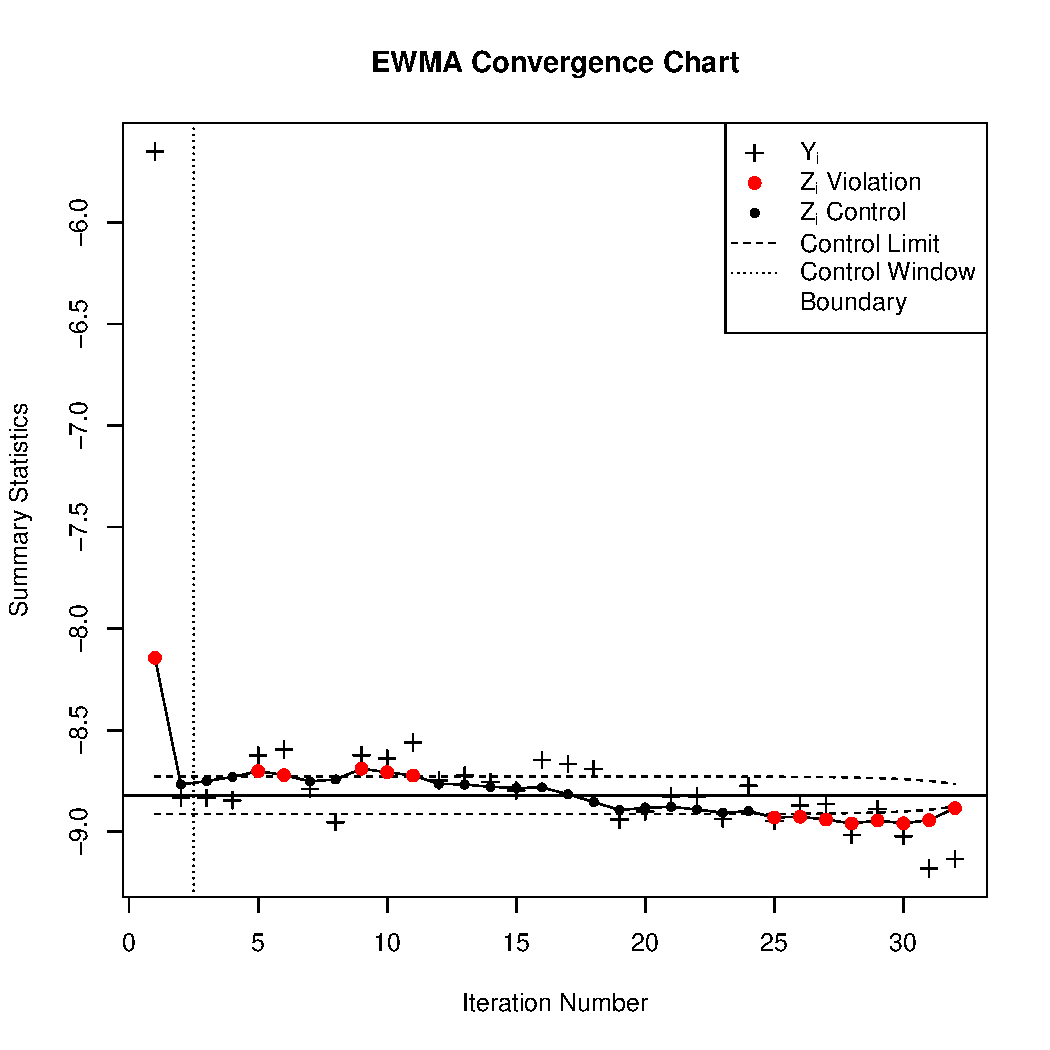
\includegraphics[width=0.49\textwidth]{ewmaConvChartRoseEasyEasyStart.pdf}
        %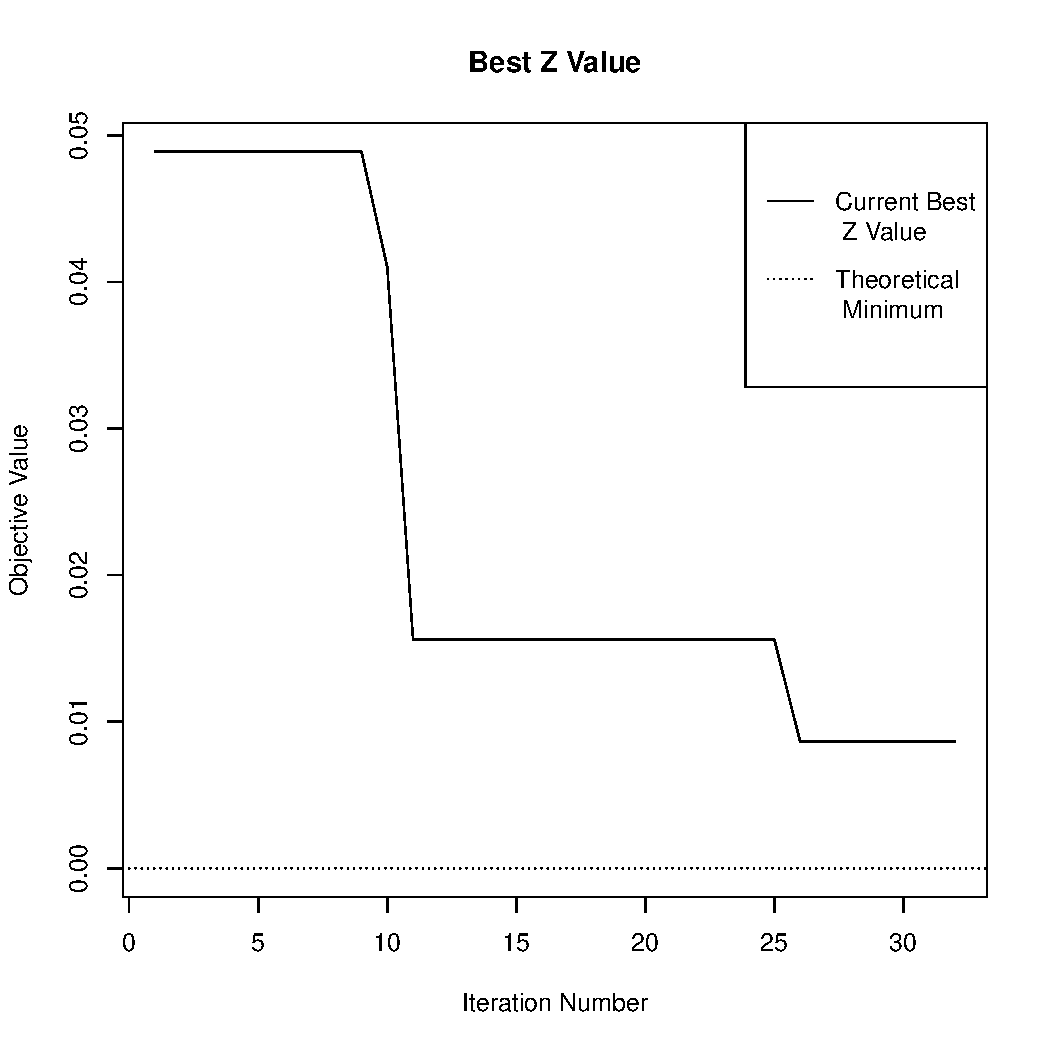
\includegraphics[width=0.49\textwidth]{bestZRoseEasyEasyStart.pdf}\\
	\includegraphics[width=0.49\textwidth]{ewmaConvChartRoseEasyEasyEnd.pdf}
        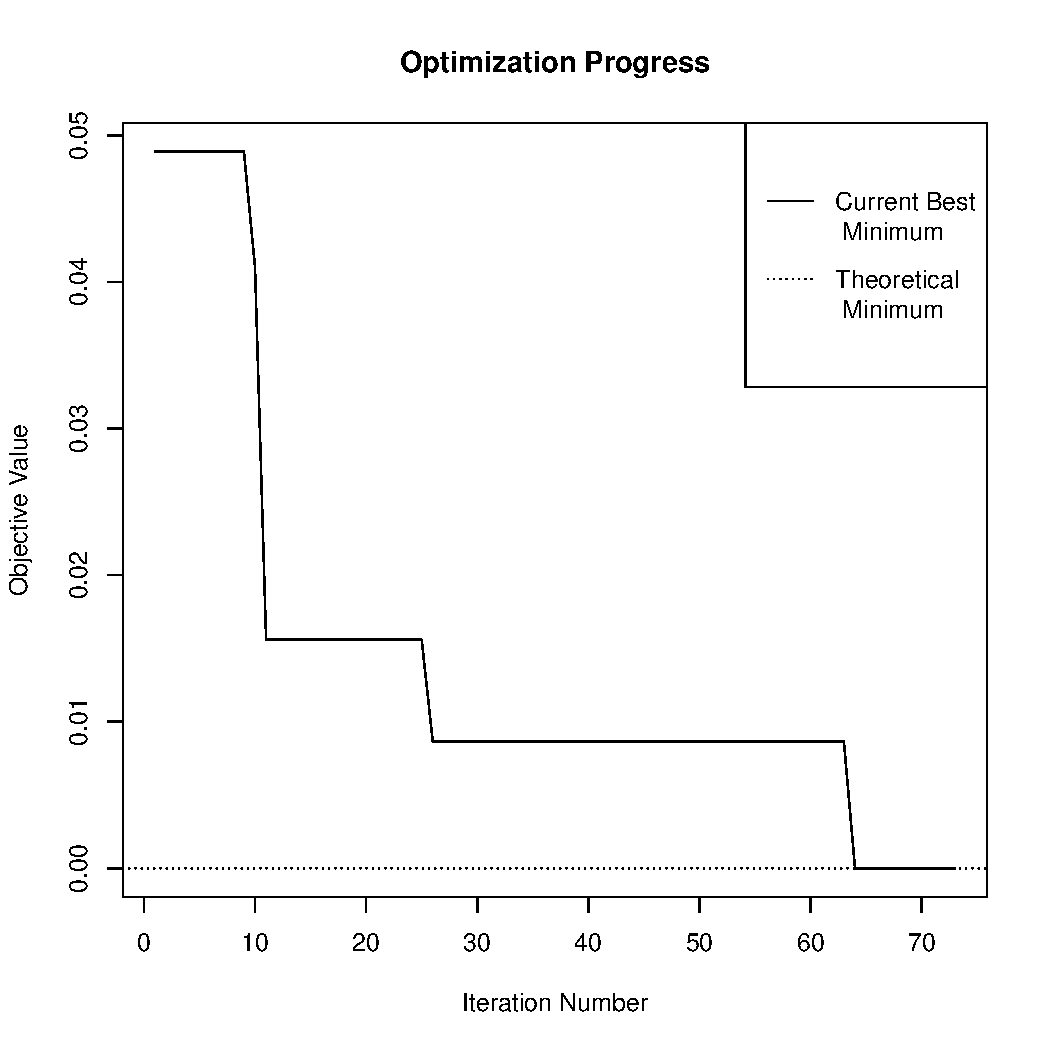
\includegraphics[width=0.49\textwidth]{bestZRoseEasyEasyEnd.pdf}
%       %\hspace{-1cm}
%       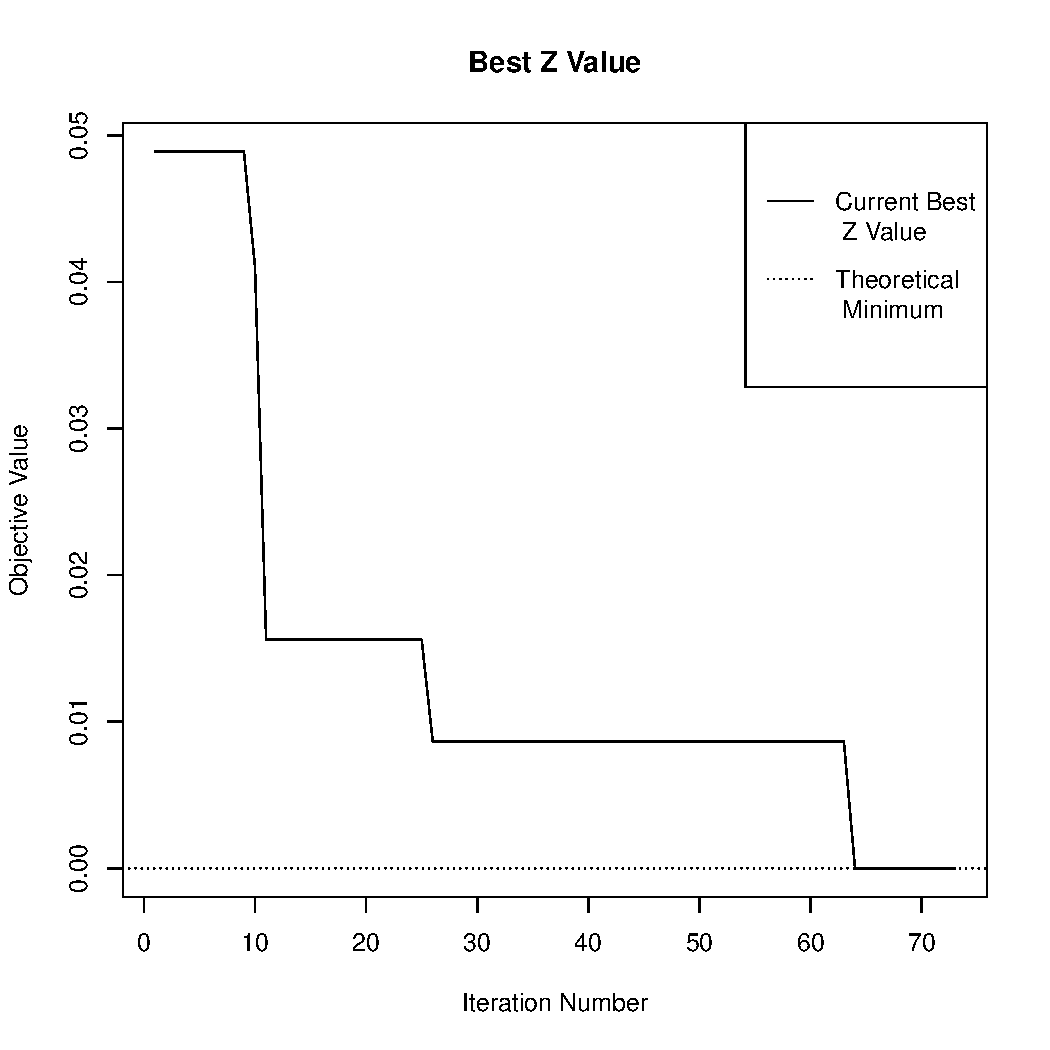
\includegraphics[width=0.245\textwidth]{./figures/bestZRoseEasyEasyEnd.pdf}
%       \includegraphics[width=0.245\textwidth]{./figures/ewmaConvChartRoseEasyEasyEnd.pdf}
        % for Rosenbrock
        %\caption{({\it left}) The initial pre-converged state of the EWMA convergence chart. ({\it right}) The cumulative smallest objective function val
        %\label{roseEWMAStart}
\end{figure}
%\begin{itemize} 
%	\item pre/post convergence chart
%	\item true optimum
%	\item other?
%\end{itemize}
\end{frame}

%
%

\subsection{}
\begin{frame}{Rastrigin Test Function}
\vspace{-0.3cm}
\begin{figure}[!h]
        \centering
        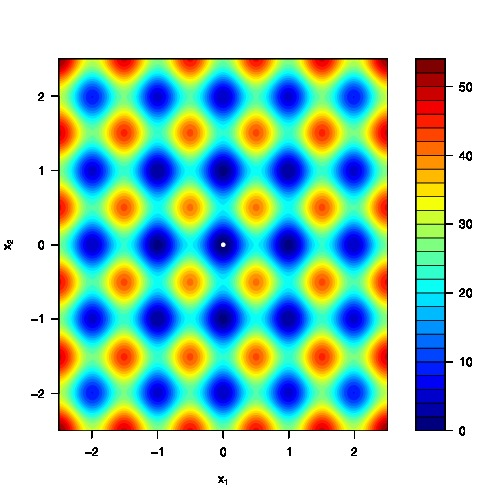
\includegraphics[width=0.49\textwidth]{rastContour.jpg}
        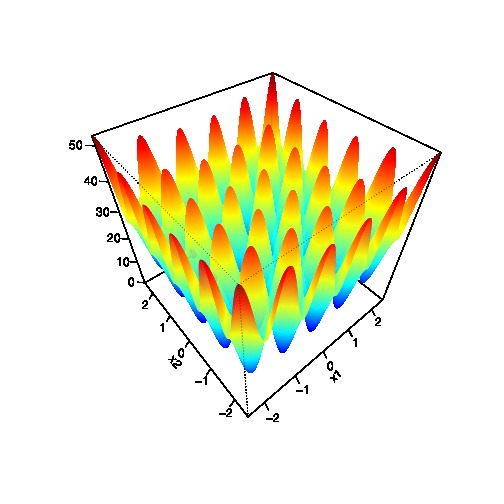
\includegraphics[width=0.49\textwidth]{rastPersp.jpg}
        \vspace{-0.5cm}
        \begin{eqnarray}
        f(x_1, x_2) &=& \sum_{i=1}^2\left[x_i^2-10\cos(2\pi x_i)\right] + 2(10)\nonumber\\
        \label{rastEq}
        \text{Minimum}&:& f(0, 0)=0\nonumber
        \end{eqnarray}
        %\begin{eqnarray}
        %f(\bm{x}) &=& 10n+\sum_{i=1}^n\left[x_i-10\cos(2\pi x_i)\right]
        %\end{eqnarray}
\end{figure}
%\begin{itemize} 
%	\item function and pictures
%	\item why its hard (genetic Al algorithm test function)
%\end{itemize}
\end{frame}

%
%

\begin{frame}{Rastrigin Pre-Convergence}
\begin{figure}[h!]%{l}{0.5\textwidth}
        %\hspace{-1cm}
        %\vspace{-0.2cm}
        %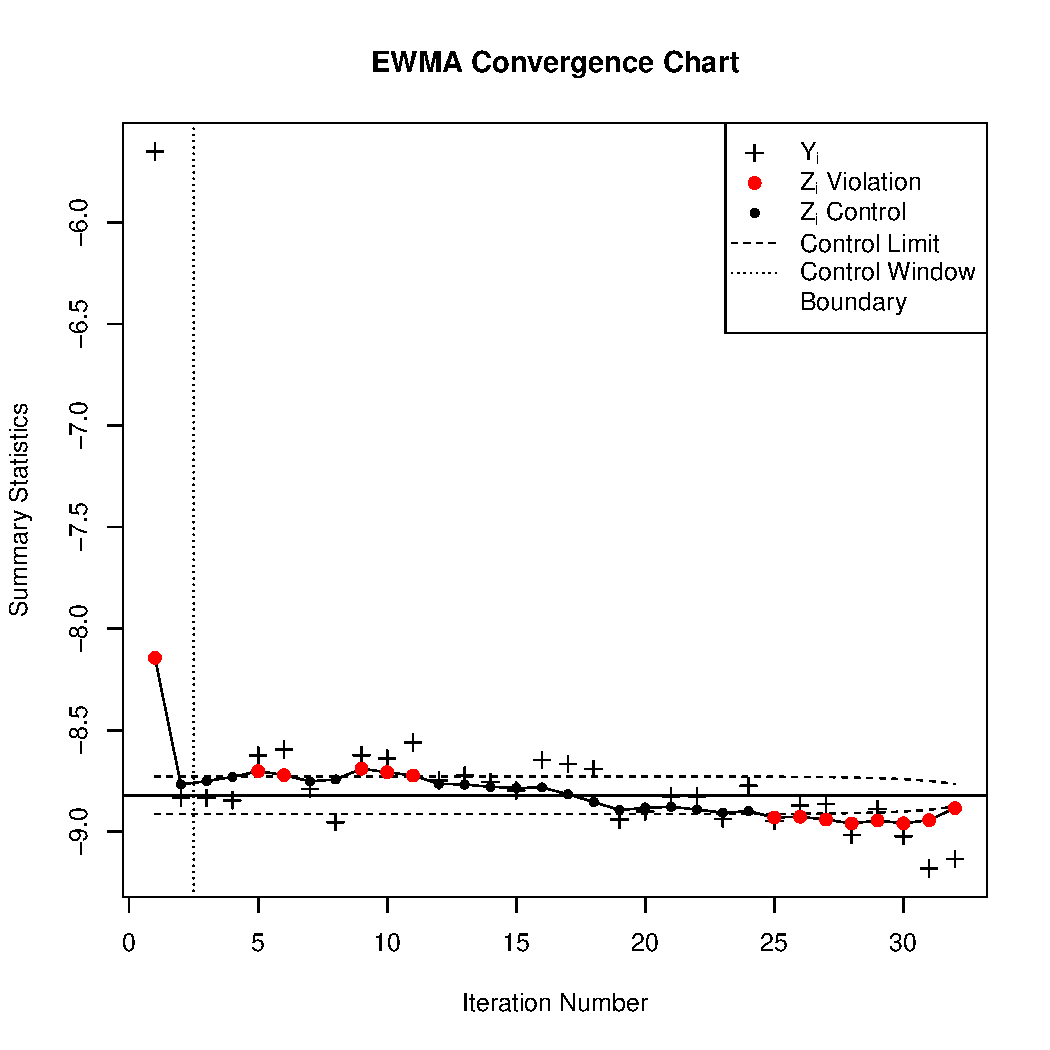
\includegraphics[width=0.49\textwidth]{ewmaConvChartRoseEasyEasyStart.pdf}
        %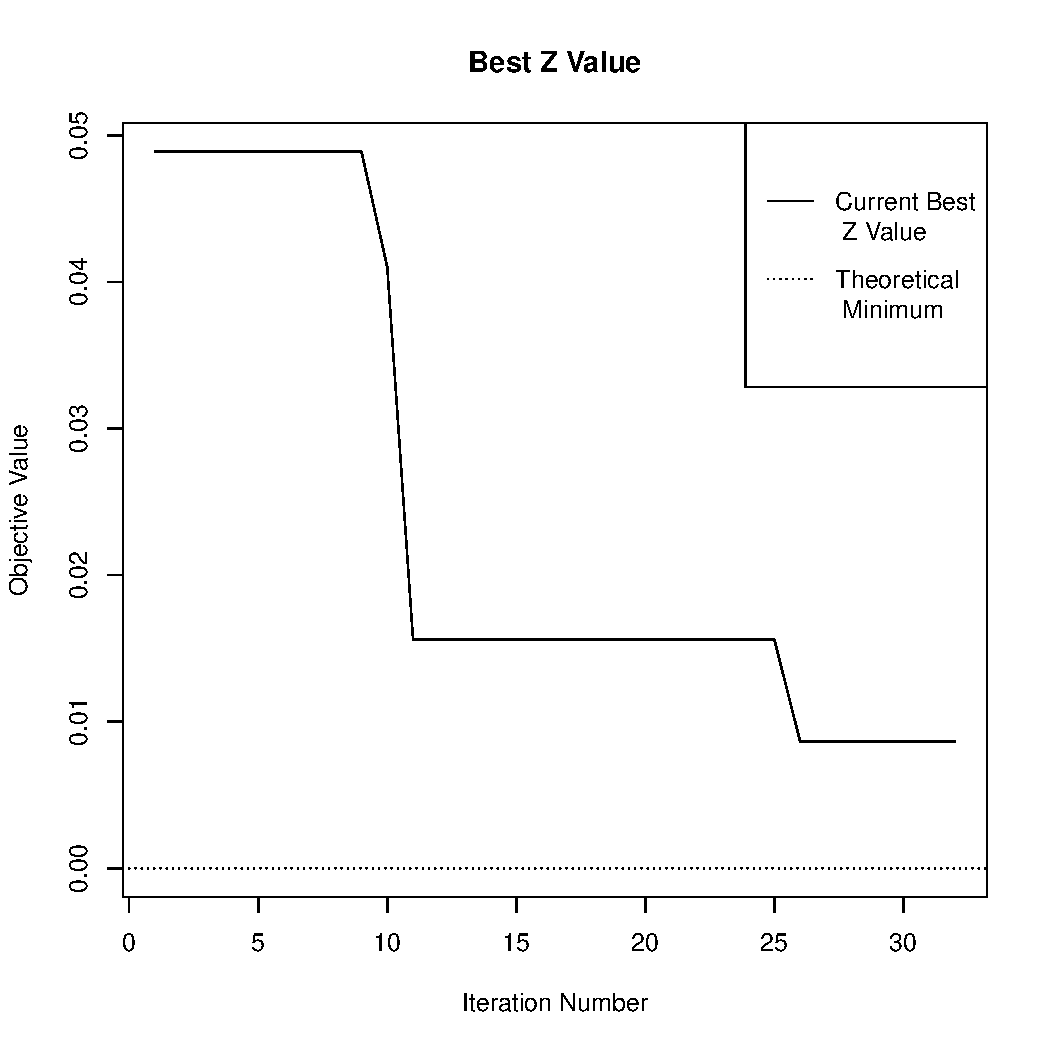
\includegraphics[width=0.49\textwidth]{bestZRoseEasyEasyStart.pdf}\\
	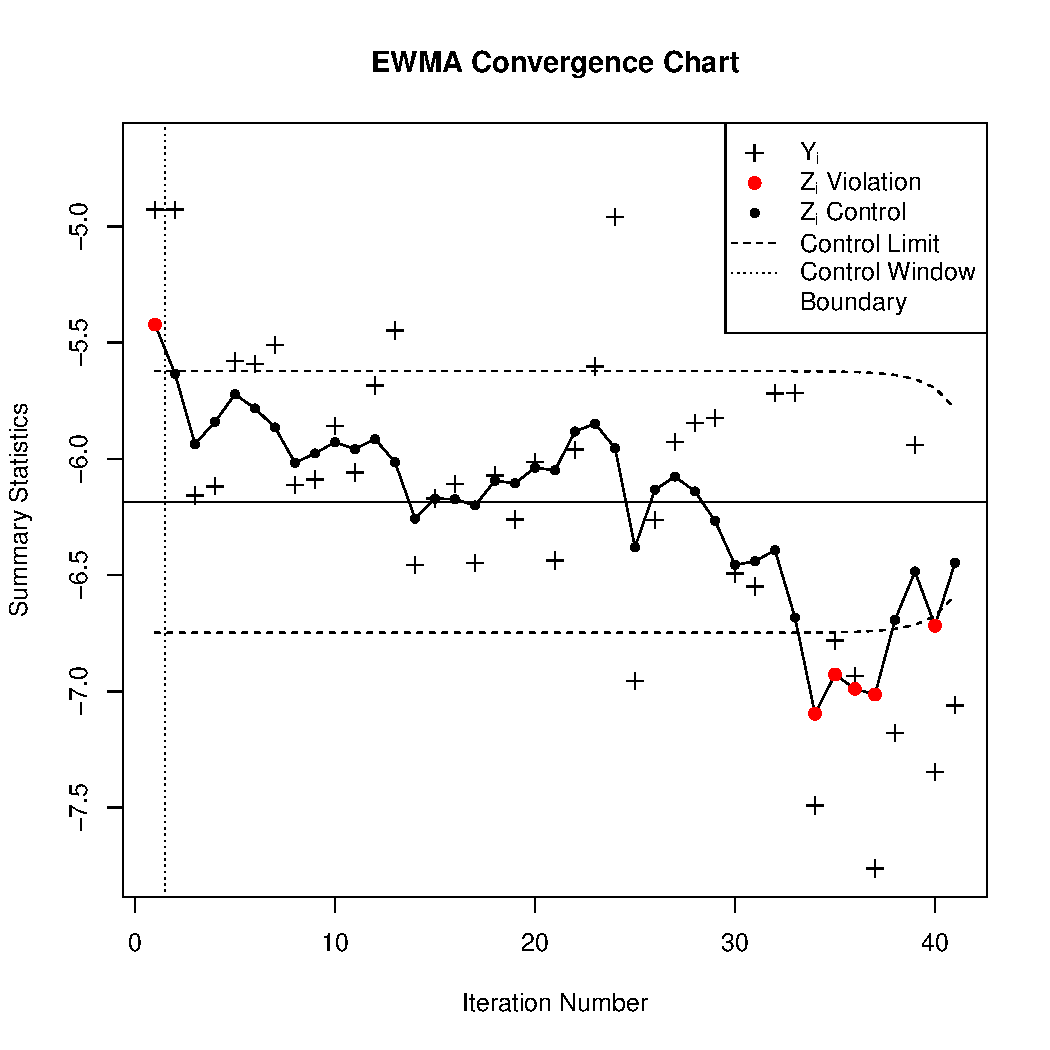
\includegraphics[width=0.49\textwidth]{ewmaConvChartRastHardStart.pdf}
        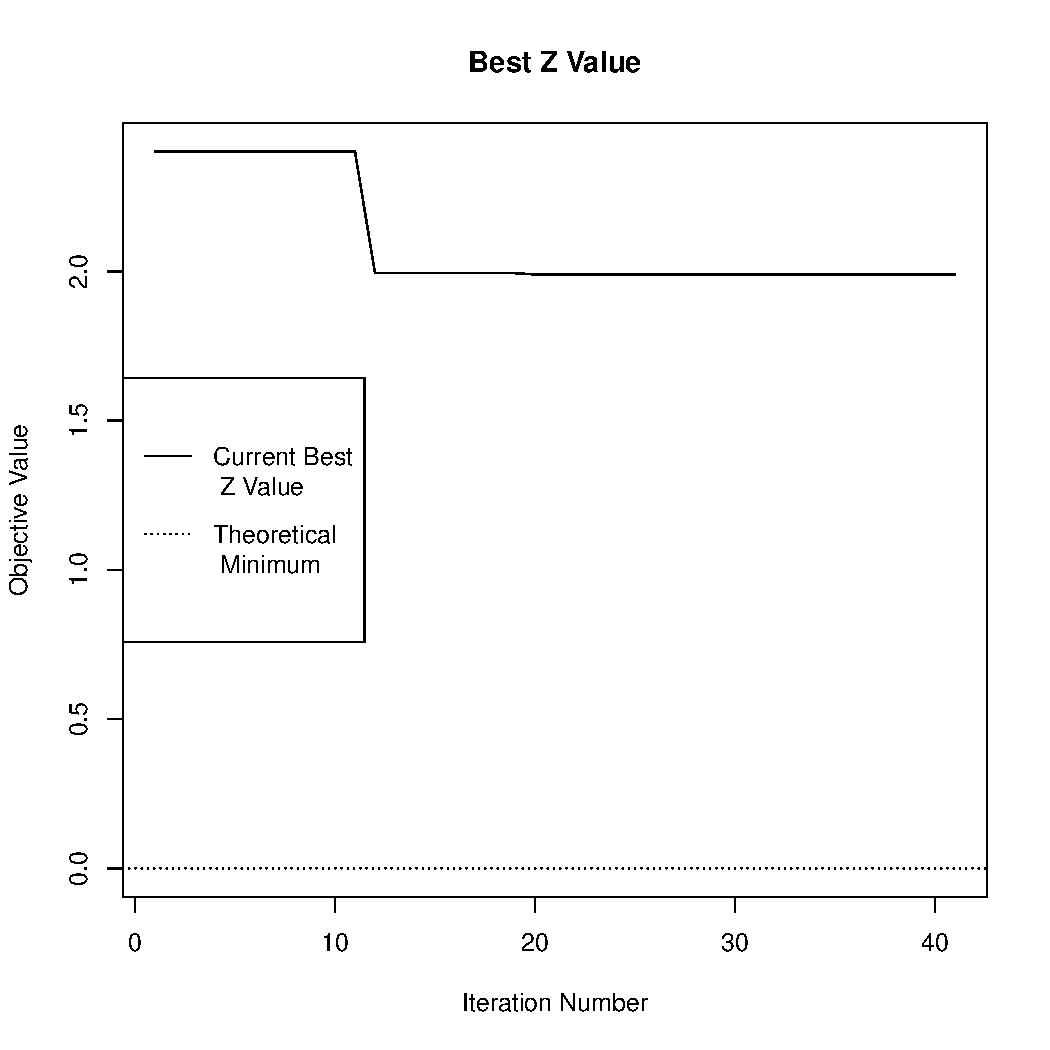
\includegraphics[width=0.49\textwidth]{bestZRastHardStart.pdf}
        %\caption{Initial EWMA convergence chart and smallest objective function value. }
        %\label{rastEWMAStart}
        %$~$\\
%       %\hspace{-1cm}
%       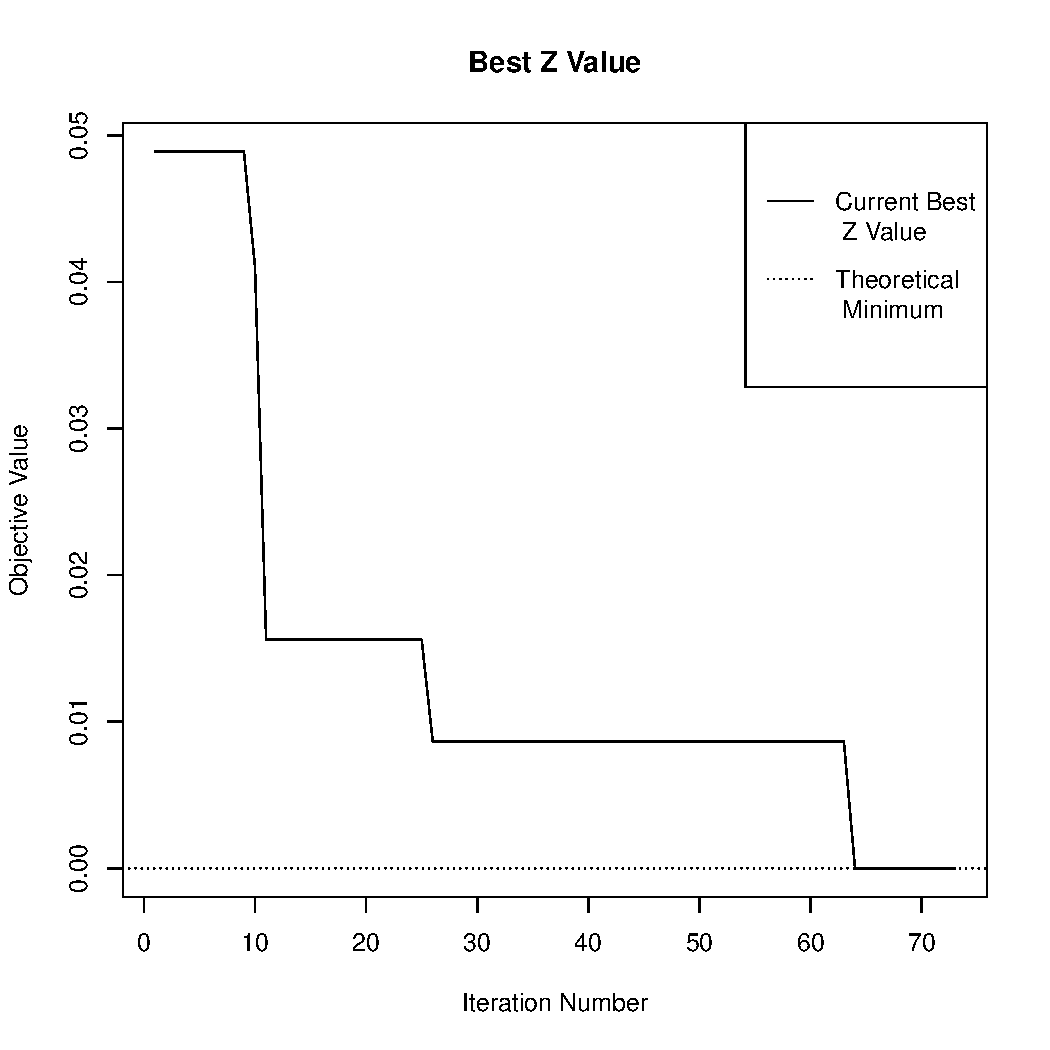
\includegraphics[width=0.245\textwidth]{./figures/bestZRoseEasyEasyEnd.pdf}
%       \includegraphics[width=0.245\textwidth]{./figures/ewmaConvChartRoseEasyEasyEnd.pdf}
        % for Rosenbrock
        %\caption{({\it left}) The initial pre-converged state of the EWMA convergence chart. ({\it right}) The cumulative smallest objective function val
        %\label{roseEWMAStart}
\end{figure}
%\begin{itemize} 
%	\item pre/post convergence chart
%	\item true optimum
%	\item other?
%\end{itemize}
\end{frame}

%
%

\begin{frame}{Rastrigin Convergence}
\begin{figure}[h!]%{l}{0.5\textwidth}
        %\hspace{-1cm}
        %\vspace{-0.2cm}
        %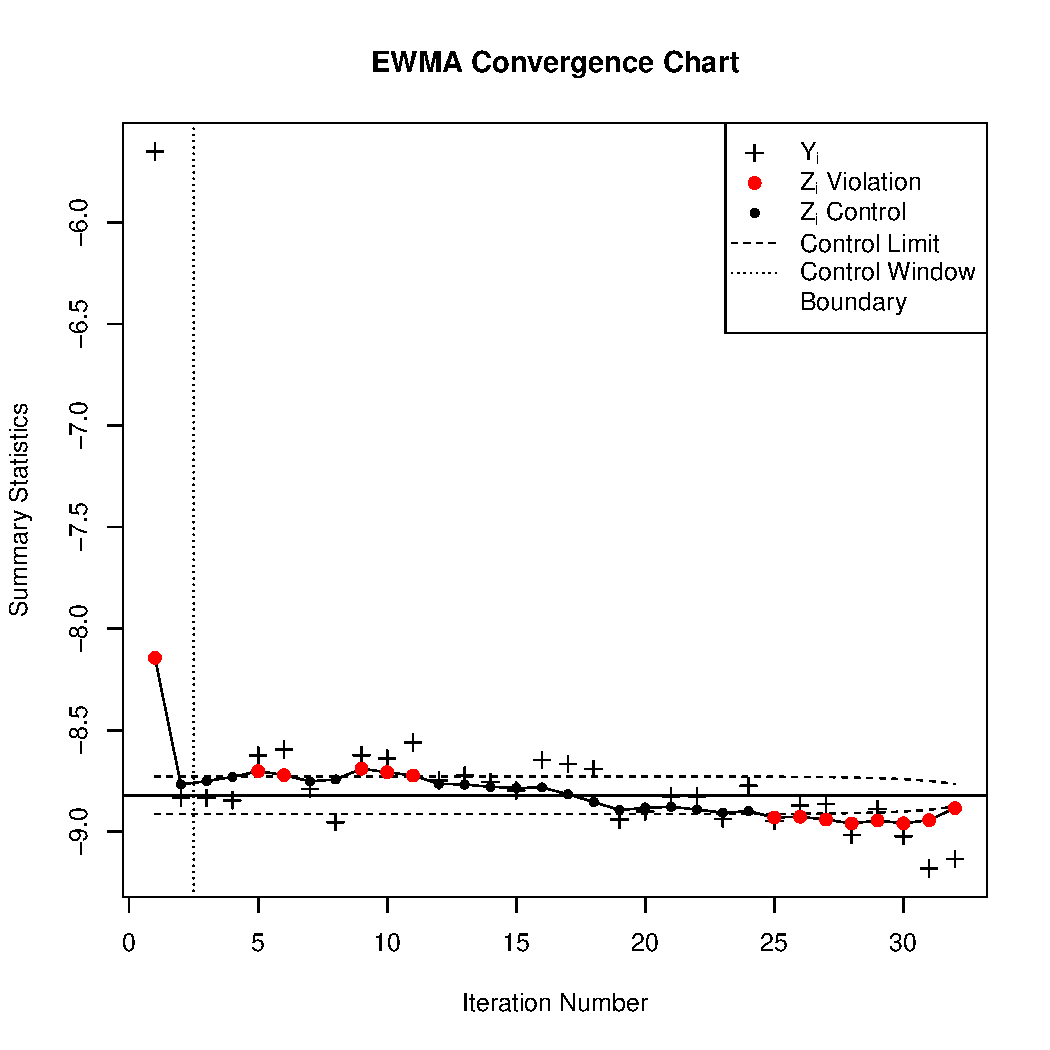
\includegraphics[width=0.49\textwidth]{ewmaConvChartRoseEasyEasyStart.pdf}
        %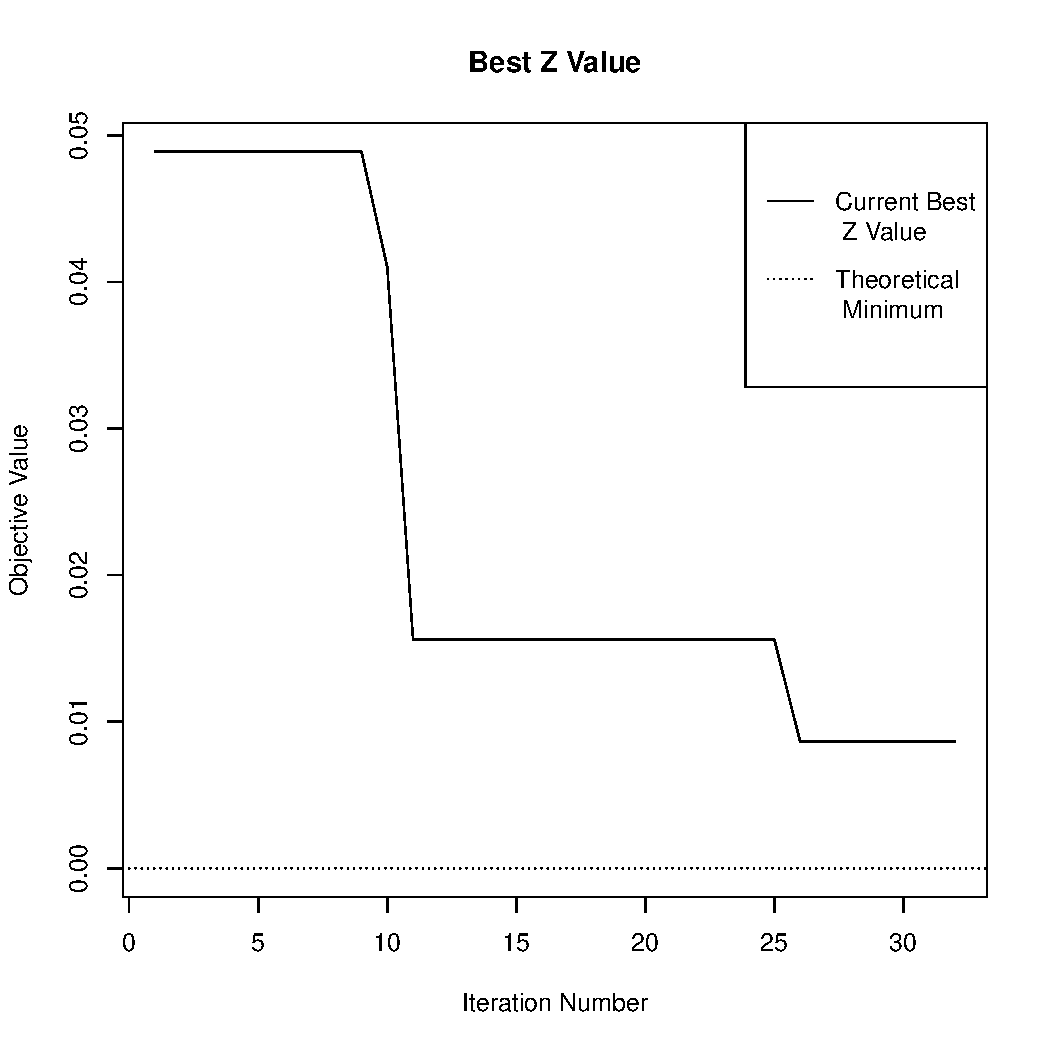
\includegraphics[width=0.49\textwidth]{bestZRoseEasyEasyStart.pdf}\\
        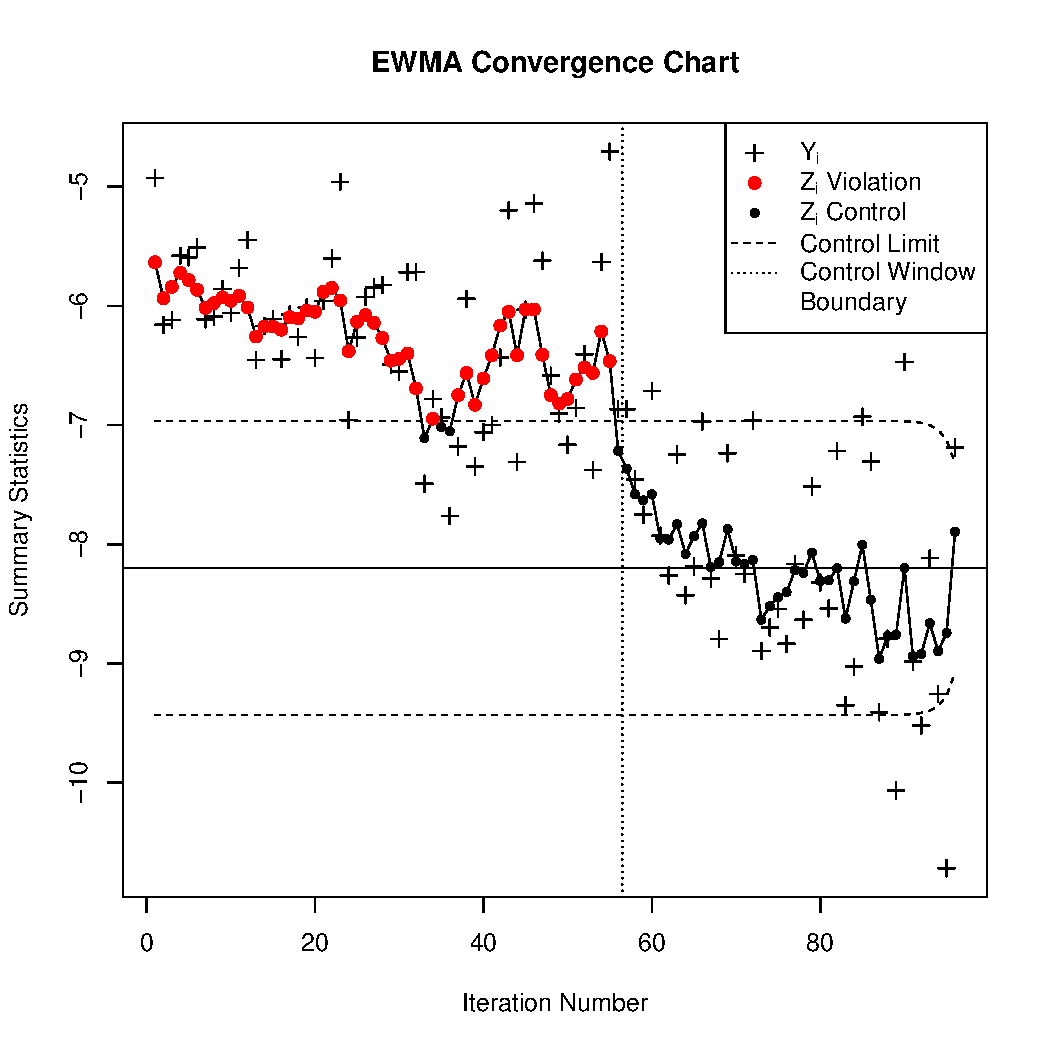
\includegraphics[width=0.49\textwidth]{ewmaConvChartRastHardEnd.pdf}
        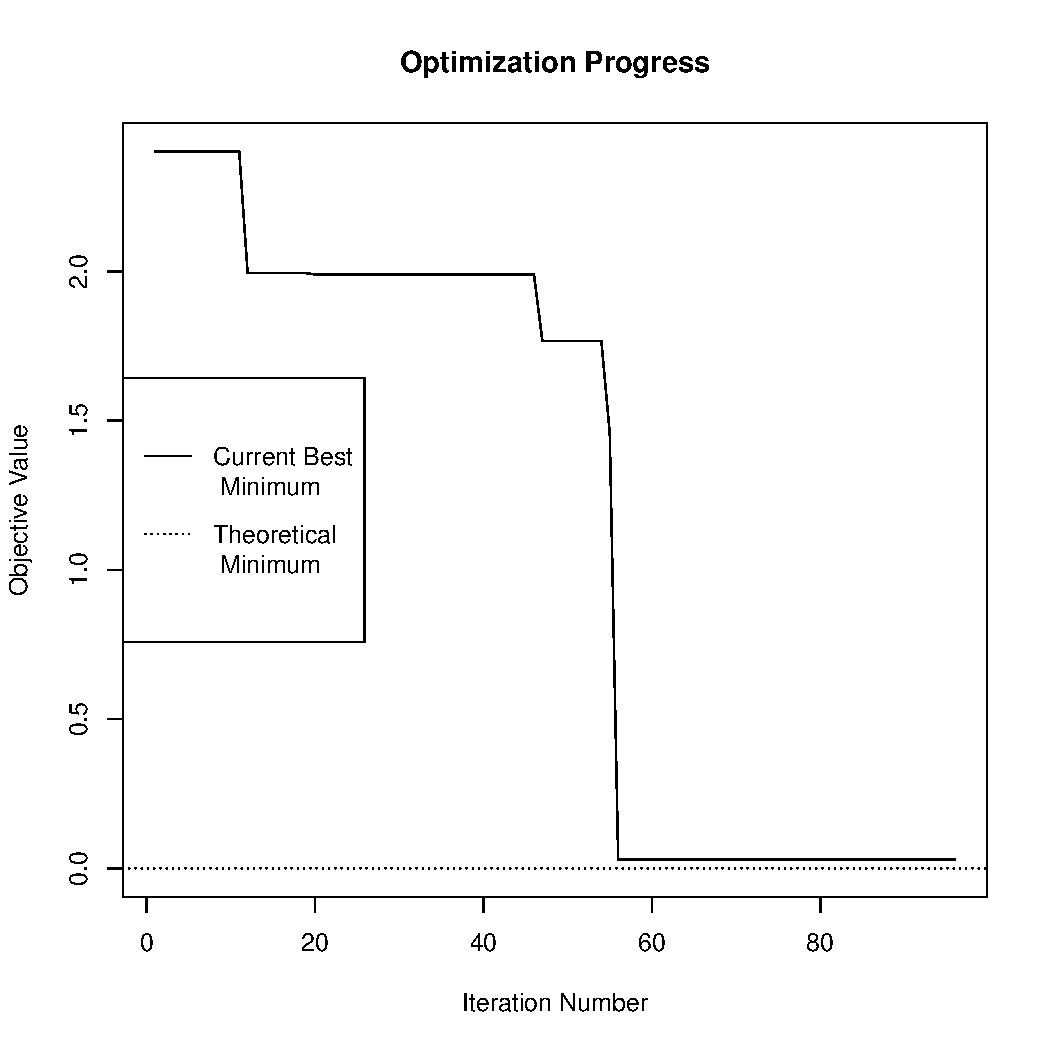
\includegraphics[width=0.49\textwidth]{bestZRastHardEnd.pdf}
        %\caption{Initial EWMA convergence chart and smallest objective function value. }
        %\label{rastEWMAStart}
        %$~$\\
%       %\hspace{-1cm}
%       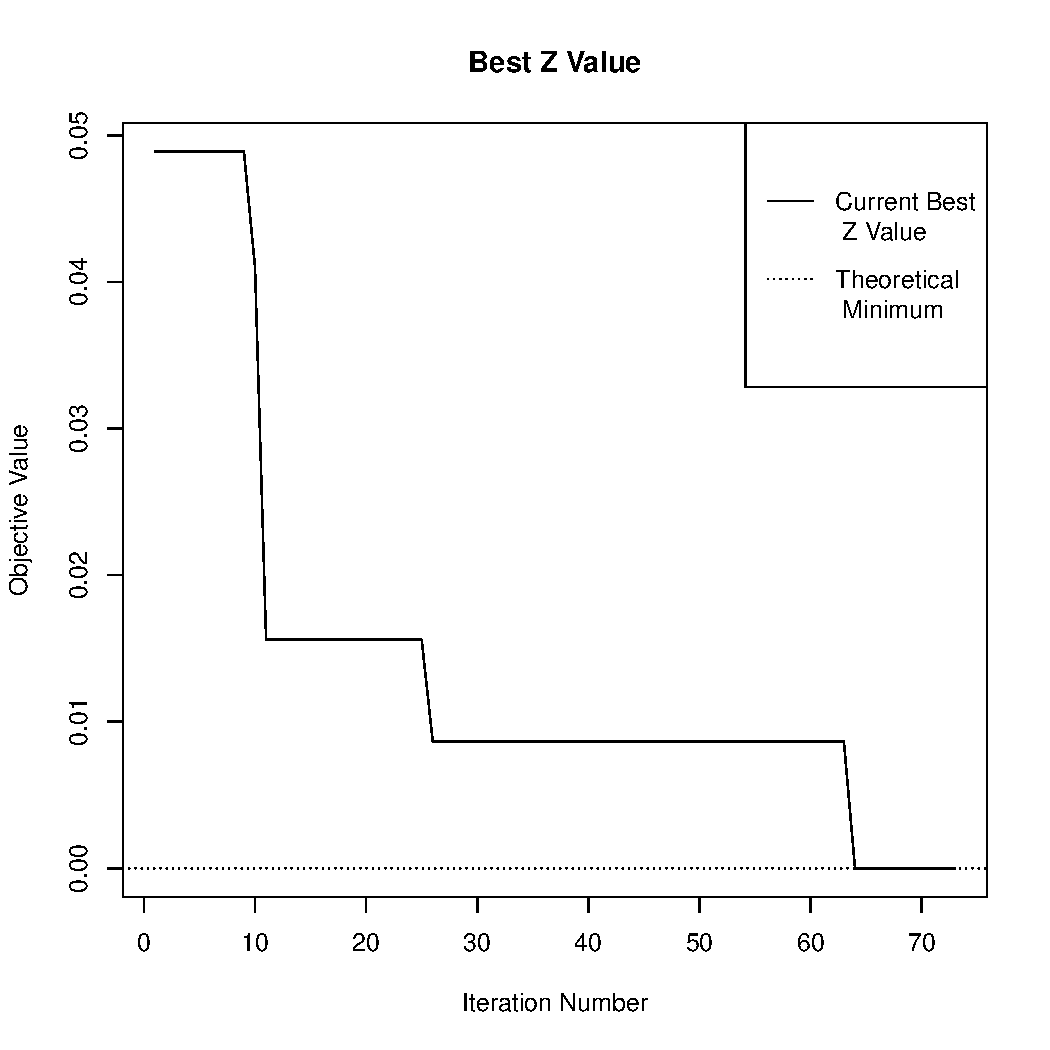
\includegraphics[width=0.245\textwidth]{./figures/bestZRoseEasyEasyEnd.pdf}
%       \includegraphics[width=0.245\textwidth]{./figures/ewmaConvChartRoseEasyEasyEnd.pdf}
        % for Rosenbrock
        %\caption{({\it left}) The initial pre-converged state of the EWMA convergence chart. ({\it right}) The cumulative smallest ob
        %\label{roseEWMAStart}
\end{figure}
%\begin{itemize} 
%       \item pre/post convergence chart
%       \item true optimum
%       \item other?
%\end{itemize}
\end{frame}


%
%

\subsection{}
\begin{frame}{Lockwood Pump-and-Treat Case Study}
\vspace{-0.3cm}
\begin{figure}[!h]
\center
\begin{minipage}[h!]{0.49\textwidth}
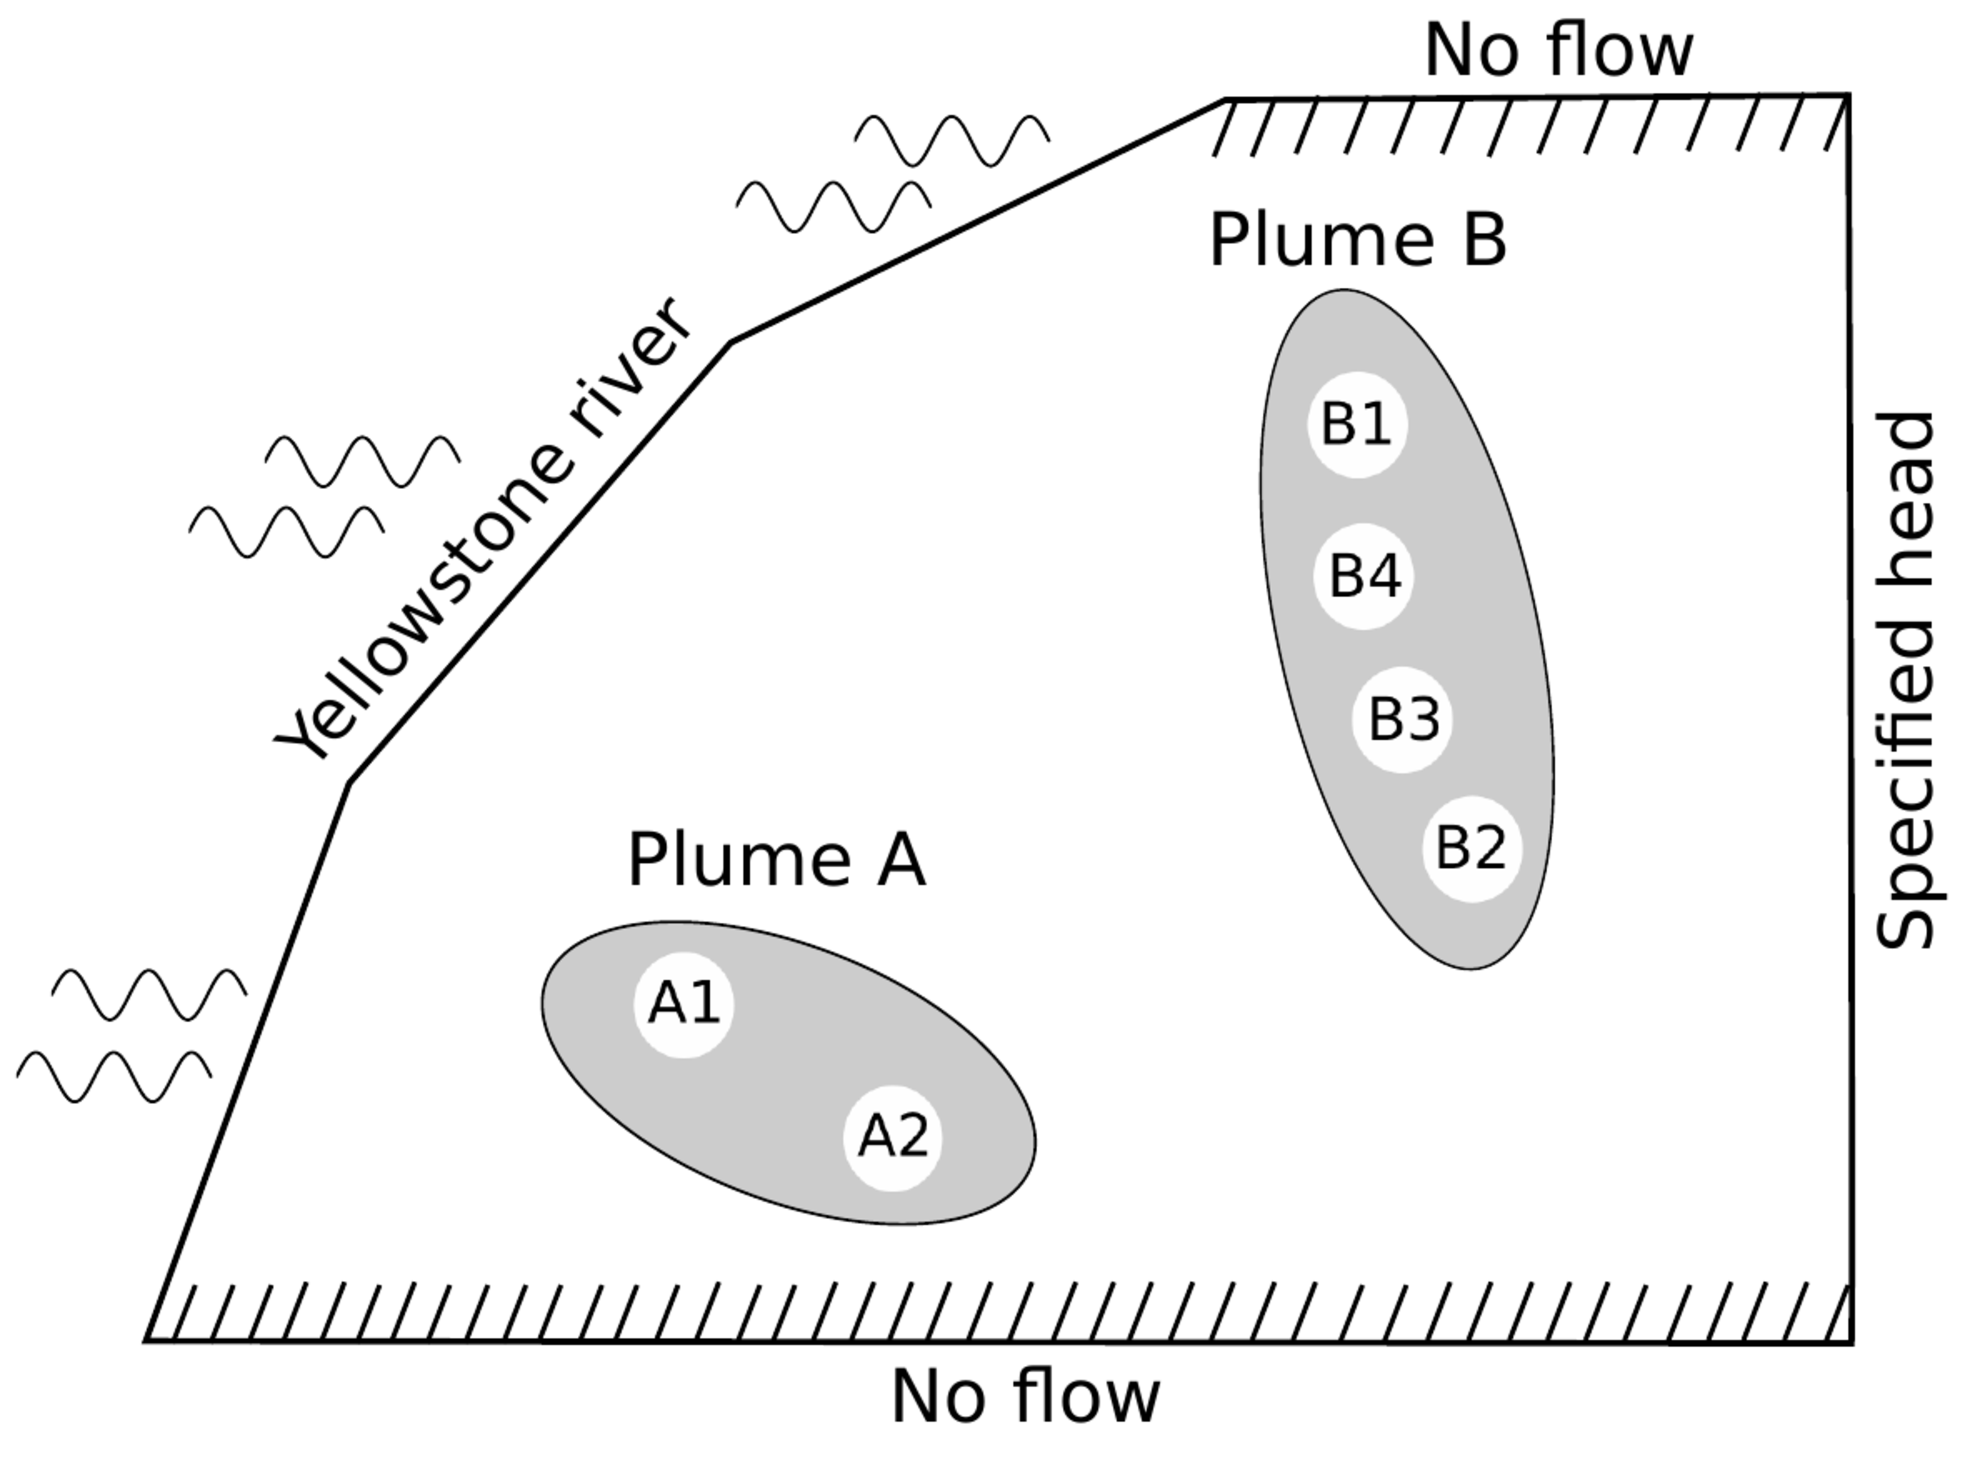
\includegraphics[width=\textwidth]{Lockwood_Site_Simple.pdf}
\end{minipage}
\begin{minipage}[h!]{0.49\textwidth}
\hspace{0.5cm}
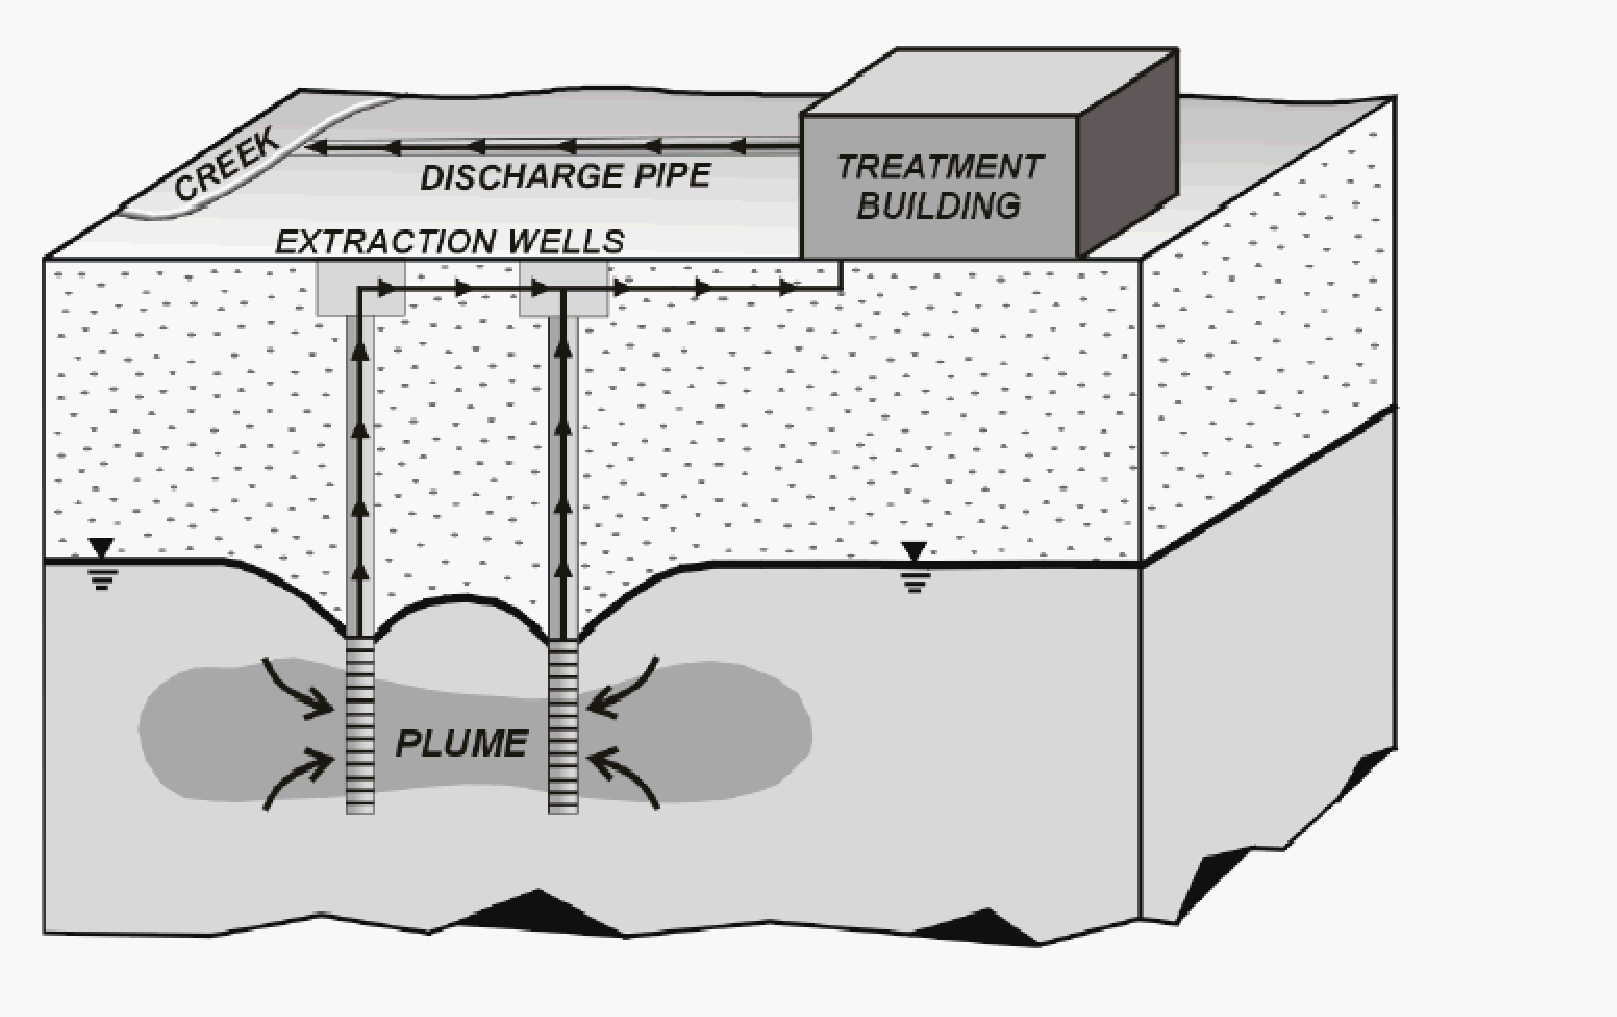
\includegraphics[width=\textwidth]{pumpandtreat.pdf}%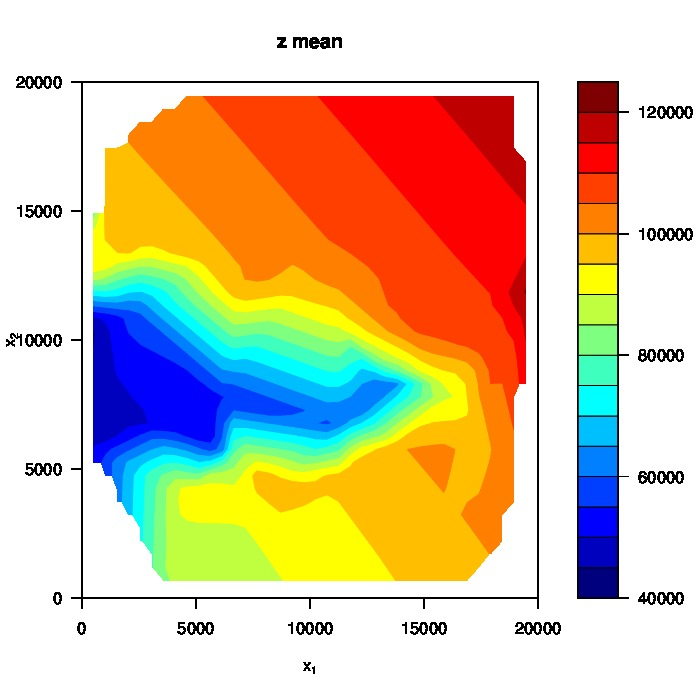
\includegraphics[width=\textwidth]{gpMeanLock240000.jpg}
\end{minipage}
%\vspace{-0.3cm}
\begin{equation*}
        f(\bm{x}) = \sum_{i=1}^6 x_i +  2\big[ c_A(\bm{x}) + c_B(\bm{x}) \big] + 20000 \big[ \oner_{c_A(\bm{x})>0} + \oner_{c_B(\bm{x})>0} \big] 
\end{equation*}
\end{figure}
%
%\begin{itemize} 
%	\item function and pictures
%	\item why its hard (dimensionality/function shape not known)
%\end{itemize}
\end{frame}

%
%

\begin{frame}{Lockwood Pre-Convergence}
\begin{figure}[h!]%{l}{0.5\textwidth}
        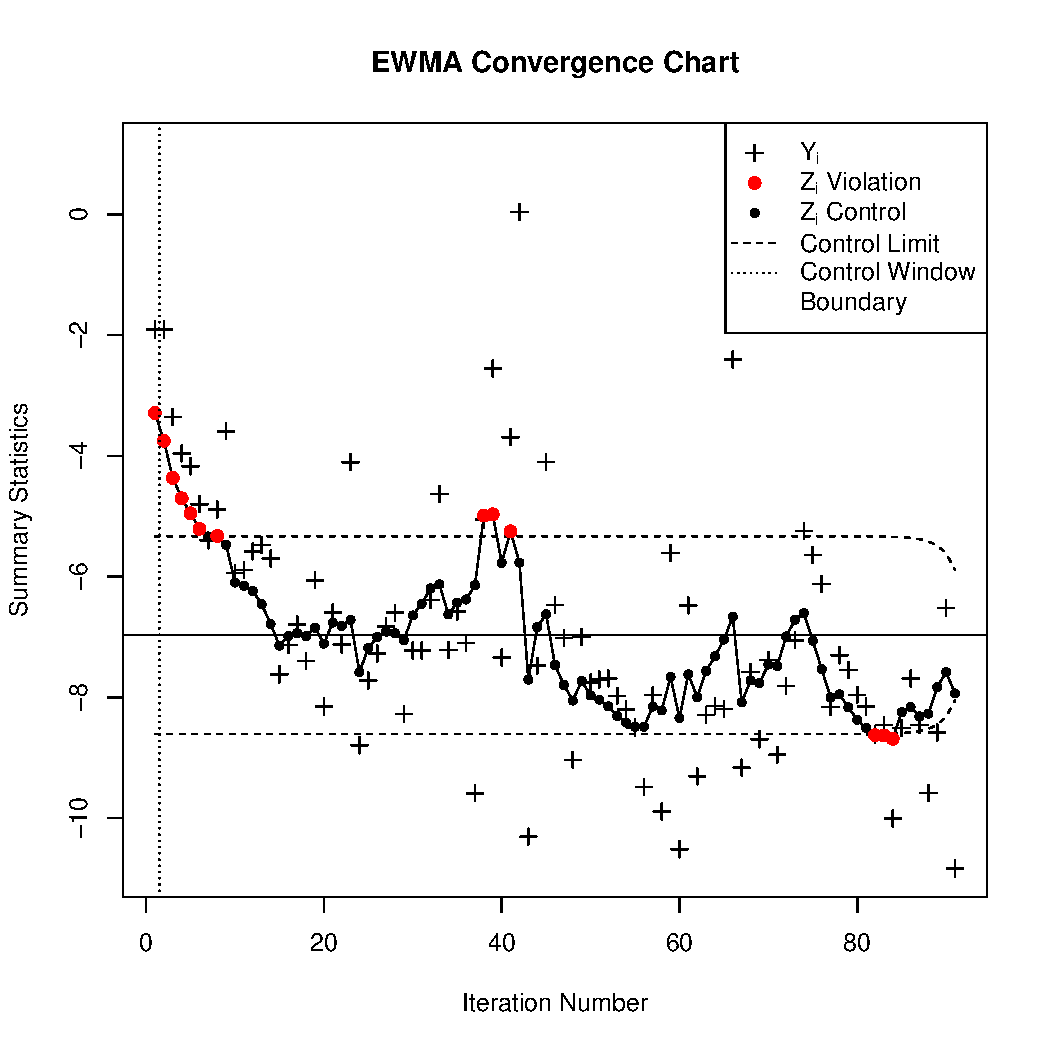
\includegraphics[width=0.49\textwidth]{ewmaConvChartLock6Three20000Start.pdf}
        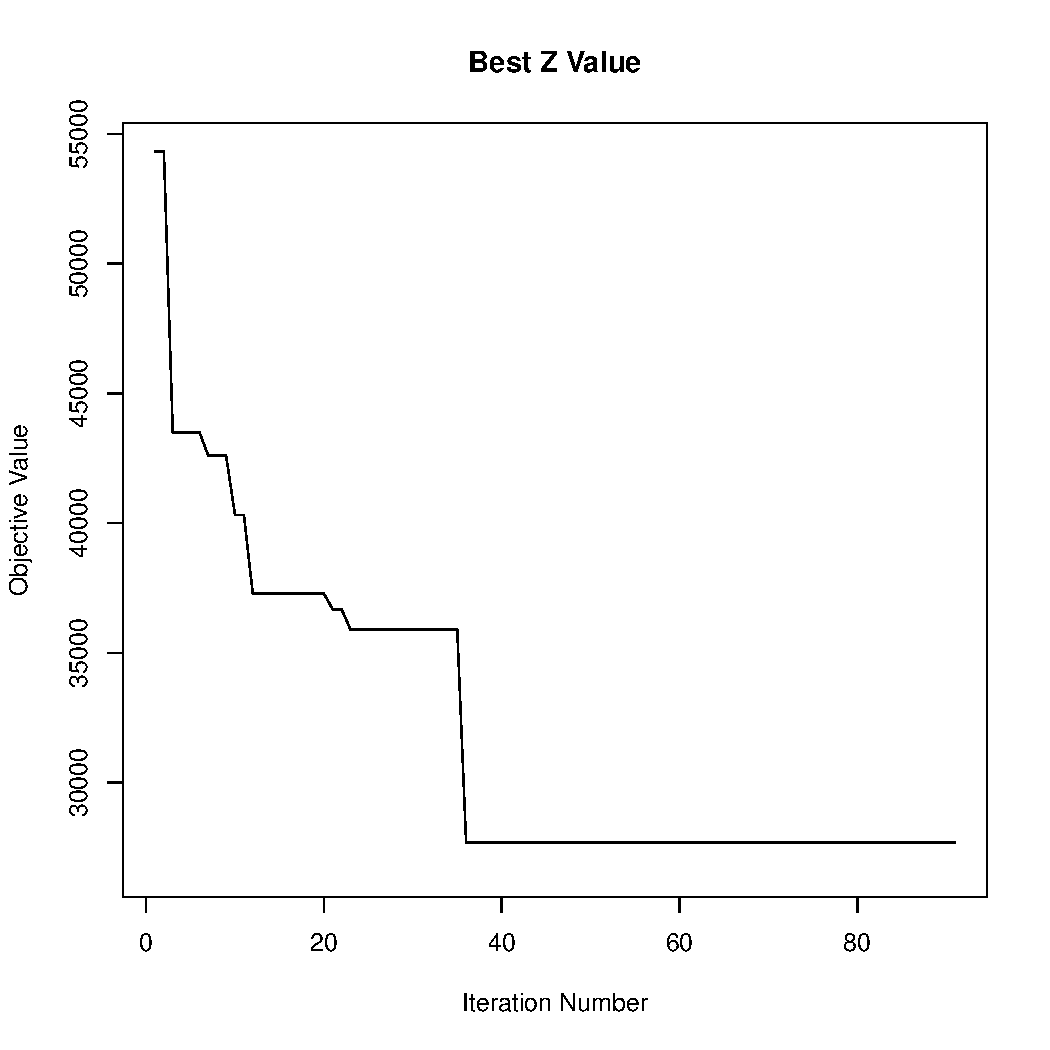
\includegraphics[width=0.49\textwidth]{bestZLock6Three20000Start.pdf}
%        \caption{Initial EWMA convergence chart and smallest objective function value. }
%        \label{easomEWMAStart}
%        $~$\\
%        \includegraphics[width=0.245\textwidth]{./figures/ewmaConvChartEasomMedEnd.pdf}
%        \includegraphics[width=0.245\textwidth]{./figures/bestZEasomMedEnd.pdf}
%        \caption{Final EWMA convergence chart and smallest objective function value. }
%        \label{easomEWMAEnd}
\end{figure}
%\begin{itemize} 
%	\item pre/post convergence chart
%	\item true optimum
%	\item other?
%\end{itemize}
\end{frame}

%
%

\begin{frame}{Lockwood Convergence}
\begin{figure}[h!]%{l}{0.5\textwidth}
        \includegraphics[width=0.49\textwidth]{ewmaConvChartLock6Three20000End.pdf}
        \includegraphics[width=0.49\textwidth]{bestZLock6Three20000End.pdf}
%        \caption{Initial EWMA convergence chart and smallest objective function value. }
%        \label{easomEWMAStart}
%        $~$\\
%        \includegraphics[width=0.245\textwidth]{./figures/ewmaConvChartEasomMedEnd.pdf}
%        \includegraphics[width=0.245\textwidth]{./figures/bestZEasomMedEnd.pdf}
%        \caption{Final EWMA convergence chart and smallest objective function value. }
%        \label{easomEWMAEnd}
\end{figure}
%\begin{itemize} 
%	\item pre/post convergence chart
%	\item true optimum
%	\item other?
%\end{itemize}
\end{frame}

\section{The End}
\subsection{}
\begin{frame}{Conclusions}
\begin{itemize} 
	\item A method for considering stochastic convergence criterion.\vspace{1cm}
	\item Convergence, in this sense, describes when surrogate modeling algorithms have exhausted their searching potential.\vspace{1cm}
	\item I want an objective way to choose the control limit size $w$. 
\end{itemize}
\end{frame}

%
%
 
\subsection{}
\begin{frame}{The Deets}
 \begin{equation*}
	%\bm{\beta}^\intercal \text{\textbf{f}}(\bm{x})
        Z(\bm{x}) = m(\bm{x}, \bm{\beta}) + \epsilon(\bm{x}) + \eta(\bm{x}).
        \label{baseEq}
\end{equation*}
\vspace{0.1cm}
        %%Here the $\bm{\beta}$ are trend parameters and  
        %Here $\eta(\bm{x})$ is Gaussian noise, and $\epsilon(\bm{x})$ is fundamentally governed by a correlation function, $ K(\bm{x}, \bm{x}')$, such that the covariance is $C(\bm{x}, \bm{x}')=\sigma^2K(\bm{x}, \bm{x}')$.
        %%the distance between \textbf{x} and \textbf{x}$'$
        %By specifying a homogeneous correlation function, we thus model the relationship of $||\bm{x}-\bm{x}'||$ with the correlation structure that we expect to see when jointly considering two such realizations of the GP.
        %%For example, tone such 
        %The following exponential power family provides a common example of such a choice of $K(\bm{x}, \bm{x}')$,
        %%
        %%
        %Considering Eq. (\ref{corrFunc}) for every combination of \textbf{x} and \textbf{x}$'$ among a particular data set provides a correlation matrix \textbf{K}; thus multiplying by $\sigma^2$ creates the likelihood covariance matrix \textbf{C}.
        %%
        %For further discussion of choices of $K(\bm{x}, \bm{x}')$ see \cite{steinBook}.
        %%% Thus we can express this model in  equations (\ref{baseEq}) and (\ref{covFunc}) together as a proper Bayesian model we get,
        %Equations (\ref{baseEq}) and (\ref{corrFunc}) imply the following simple Bayesian model, which forms the basis for many other complex GP models
        %%
\begin{equation*}
        \begin{aligned}
        \text{\textbf{Z}} ~|~ \bm{\beta}, \sigma^2, \text{\textbf{K}} &~\sim~ N_n\Big(\text{\textbf{F}}\bm{\beta},~ \sigma^2\text{\textbf{K}}\Big)
        &~ \sigma^2 &~\sim~ IG\left(\frac{\alpha_\sigma}{2}, ~\frac{\beta_\sigma}{2}\right)
        \\
        \bm{\beta} ~|~ \sigma^2, \tau^2, \bm{\beta}_0, \text{\textbf{W}} &~\sim~ N_m\Big(\bm{\beta}_0,~ \sigma^2\tau^2\text{\textbf{W}}\Big) &~
	\tau^2 &~\sim~ IG\left(\frac{\alpha_\tau}{2}, ~\frac{\beta_\tau}{2}\right)
        \\
	\bm{\beta}_0 &~\sim~ N_m\Big( \bm{\mu}, ~\text{\textbf{B}} \Big) &~
	\text{\textbf{W}} &~\sim~ IW\big(\rho\bm{V}, ~\rho\big).
        \label{gpModel}
        \end{aligned}
\end{equation*}

\begin{equation*}
        K(\bm{x}_j, \bm{x}_k|d) = \exp\left\{ -\frac{||\bm{x}_j-\bm{x}_k||^p}{d} \right\} + g \delta_{j,k}
\end{equation*}

\end{frame}

\begin{frame}{}%\color{red} Choosing Parameters} 
\begin{center}
%\vspace{-0.5cm}
\includegraphics[height=\textheight]{ssRastHardOpt.pdf}
\end{center}
%\begin{itemize}
%        \item Minimum SSFE $\lambda$ estimator
%        \item $w$
%	\item outline the $w$ descision dynamics
%\end{itemize}
\end{frame}

\end{document}
